\documentclass[]{article}
%DIF LATEXDIFF DIFFERENCE FILE
%DIF DEL doc/manuscript_submitted_raw.tex   Mon Jul 24 18:06:15 2017
%DIF ADD doc/manuscript_new_raw.tex         Mon Jul 24 18:07:18 2017
\usepackage{lmodern}
\usepackage{amssymb,amsmath}
\usepackage{ifxetex,ifluatex}
\usepackage{fixltx2e} % provides \textsubscript
\ifnum 0\ifxetex 1\fi\ifluatex 1\fi=0 % if pdftex
  \usepackage[T1]{fontenc}
  \usepackage[utf8]{inputenc}
\else % if luatex or xelatex
  \ifxetex
    \usepackage{mathspec}
  \else
    \usepackage{fontspec}
  \fi
  \defaultfontfeatures{Ligatures=TeX,Scale=MatchLowercase}
\fi
% use upquote if available, for straight quotes in verbatim environments
\IfFileExists{upquote.sty}{\usepackage{upquote}}{}
% use microtype if available
\IfFileExists{microtype.sty}{%
\usepackage{microtype}
\UseMicrotypeSet[protrusion]{basicmath} % disable protrusion for tt fonts
}{}
\usepackage[a4paper]{geometry}
\usepackage[unicode=true]{hyperref}
\hypersetup{
            pdftitle={Dipolar~extracellular~potentials generated~by~axonal~projections},
            pdfauthor={Thomas McColgan,; Ji Liu,; Paula T Kuokkanen,; Catherine E Carr,; Hermann Wagner,; Richard Kempter},
            pdfborder={0 0 0},
            breaklinks=true}
\urlstyle{same}  % don't use monospace font for urls
%DIF 32a32
\usepackage{longtable,booktabs} %DIF > 
%DIF -------
\usepackage{graphicx,grffile}
\makeatletter
\def\maxwidth{\ifdim\Gin@nat@width>\linewidth\linewidth\else\Gin@nat@width\fi}
\def\maxheight{\ifdim\Gin@nat@height>\textheight\textheight\else\Gin@nat@height\fi}
\makeatother
% Scale images if necessary, so that they will not overflow the page
% margins by default, and it is still possible to overwrite the defaults
% using explicit options in \includegraphics[width, height, ...]{}
\setkeys{Gin}{width=\maxwidth,height=\maxheight,keepaspectratio}
\IfFileExists{parskip.sty}{%
\usepackage{parskip}
}{% else
\setlength{\parindent}{0pt}
\setlength{\parskip}{6pt plus 2pt minus 1pt}
}
\setlength{\emergencystretch}{3em}  % prevent overfull lines
\providecommand{\tightlist}{%
  \setlength{\itemsep}{0pt}\setlength{\parskip}{0pt}}
\setcounter{secnumdepth}{0}
% Redefines (sub)paragraphs to behave more like sections
\ifx\paragraph\undefined\else
\let\oldparagraph\paragraph
\renewcommand{\paragraph}[1]{\oldparagraph{#1}\mbox{}}
\fi
\ifx\subparagraph\undefined\else
\let\oldsubparagraph\subparagraph
\renewcommand{\subparagraph}[1]{\oldsubparagraph{#1}\mbox{}}
\fi
\usepackage{setspace}
\doublespacing
\usepackage{lineno}
\linenumbers
\usepackage{subfig}
\AtBeginDocument{%
\renewcommand*\figurename{Figure}
\renewcommand*\tablename{Table}
}
\AtBeginDocument{%
\renewcommand*\listfigurename{List of Figures}
\renewcommand*\listtablename{List of Tables}
}
\usepackage{float}
\floatstyle{ruled}
\makeatletter
\@ifundefined{c@chapter}{\newfloat{codelisting}{h}{lop}}{\newfloat{codelisting}{h}{lop}[chapter]}
\makeatother
\floatname{codelisting}{Listing}
\newcommand*\listoflistings{\listof{codelisting}{List of Listings}}

\title{Dipolar~extracellular~potentials generated~by~axonal~projections}
\author{Thomas
McColgan,\footnote{Department of Biology, Institute of Theoretical Biology, Humboldt-Universität zu Berlin, Berlin, Germany} \and Ji
Liu,\footnote{Department of Biology, University of Maryland, College Park, MD, USA} \and Paula T Kuokkanen,\footnotemark[1] \footnotemark[2] \and Catherine E Carr,\footnotemark[2] \and Hermann
Wagner,\footnote{Institute for Biology II, RWTH Aachen, Aachen, Germany} \and Richard
Kempter\footnotemark[1] \footnote{Bernstein Center for Computational Neuroscience, Berlin, Germany}
\footnote{Einstein Center for Neurosciences, Berlin, Germany}}
\date{}
%DIF PREAMBLE EXTENSION ADDED BY LATEXDIFF
%DIF UNDERLINE PREAMBLE %DIF PREAMBLE
\RequirePackage[normalem]{ulem} %DIF PREAMBLE
\RequirePackage{color}\definecolor{RED}{rgb}{1,0,0}\definecolor{BLUE}{rgb}{0,0,1} %DIF PREAMBLE
\providecommand{\DIFaddtex}[1]{{\protect\color{blue}\uwave{#1}}} %DIF PREAMBLE
\providecommand{\DIFdeltex}[1]{{\protect\color{red}\sout{#1}}}                      %DIF PREAMBLE
%DIF SAFE PREAMBLE %DIF PREAMBLE
\providecommand{\DIFaddbegin}{} %DIF PREAMBLE
\providecommand{\DIFaddend}{} %DIF PREAMBLE
\providecommand{\DIFdelbegin}{} %DIF PREAMBLE
\providecommand{\DIFdelend}{} %DIF PREAMBLE
%DIF FLOATSAFE PREAMBLE %DIF PREAMBLE
\providecommand{\DIFaddFL}[1]{\DIFadd{#1}} %DIF PREAMBLE
\providecommand{\DIFdelFL}[1]{\DIFdel{#1}} %DIF PREAMBLE
\providecommand{\DIFaddbeginFL}{} %DIF PREAMBLE
\providecommand{\DIFaddendFL}{} %DIF PREAMBLE
\providecommand{\DIFdelbeginFL}{} %DIF PREAMBLE
\providecommand{\DIFdelendFL}{} %DIF PREAMBLE
%DIF END PREAMBLE EXTENSION ADDED BY LATEXDIFF
%DIF PREAMBLE EXTENSION ADDED BY LATEXDIFF
%DIF HYPERREF PREAMBLE %DIF PREAMBLE
\providecommand{\DIFadd}[1]{\texorpdfstring{\DIFaddtex{#1}}{#1}} %DIF PREAMBLE
\providecommand{\DIFdel}[1]{\texorpdfstring{\DIFdeltex{#1}}{}} %DIF PREAMBLE
%DIF END PREAMBLE EXTENSION ADDED BY LATEXDIFF

\begin{document}
\maketitle
\begin{abstract}
Extracellular field potentials (EFPs) are an important source of
information in neuroscience, but their physiological basis is in many
cases still a matter of debate. Axonal sources are typically discounted
in modeling and data analysis because their contributions are assumed to
be negligible. Here, we \DIFdelbegin \DIFdel{show }\DIFdelend \DIFaddbegin \DIFadd{established }\DIFaddend experimentally and theoretically
that contributions of axons to EFPs can be significant. Modeling action
potentials propagating along axons, we showed that EFPs were prominent
in the presence of \DIFdelbegin \DIFdel{a terminal zone }\DIFdelend \DIFaddbegin \DIFadd{terminal zones }\DIFaddend where axons branch and terminate in
close succession, as found in many brain regions. Our models predicted a
dipolar far field and a polarity reversal at the center of the terminal
zone. We confirmed these predictions using EFPs from the barn owl
auditory brainstem where we recorded in nucleus laminaris using a
multielectrode array. These results demonstrate that axonal terminal
zones \DIFaddbegin \DIFadd{can }\DIFaddend produce EFPs with considerable amplitude and spatial reach.
\end{abstract}

\section{Introduction}\label{introduction}

Extracellular field potentials (EFPs) are at the heart of many
experimental approaches used to examine the inner workings of the brain.
Types of EFPs include invasively recorded signals such as the
electrocorticogram (ECoG) \DIFdelbegin \DIFdel{, }\DIFdelend \DIFaddbegin \DIFadd{and }\DIFaddend the local field potential (LFP), \DIFdelbegin \DIFdel{the current
source density (CSD), and the multiunit activity (MUA) }\DIFdelend as well
as the noninvasively recorded electroencephalogram (EEG) and the
auditory brainstem response (ABR) (Nunez and Srinivasan, 2006; Brette
and Destexhe, 2012). \DIFaddbegin \DIFadd{Measures derived from the EFP such as the current
source density (CSD) and multiunit activity (MUA) are also frequently
used. }\DIFaddend The origins of these signals \DIFaddbegin \DIFadd{and measures}\DIFaddend , especially in cases in
which the activity is not clearly attributable to a single cell, is a
matter of debate (Buzsáki et al., 2012).

EFPs in the brain were long thought to be primarily of synaptic origin
(Buzsáki et al., 2012). As a consequence, many modeling studies focussed
on the extracellular fields induced by postsynaptic currents on the
dendrites and the soma of a neuron (Holt and Koch, 1999; Lindén et al.,
2010, 2011; Einevoll et al., 2013; Fernández-Ruiz et al., 2013).
However, a number of recent data analyses and modeling efforts have
revealed that active, non-synaptic membrane currents can play an
important role in generating population-level EFPs (\DIFaddbegin \DIFadd{Reichinnek et al.,
2010; }\DIFaddend Ray and Maunsell, 2011; Belluscio et al., 2012; Schomburg et al.,
2012; Reimann et al., 2013; \DIFaddbegin \DIFadd{Scheffer-Teixeira et al., 2013; }\DIFaddend Waldert et
al., 2013; Anastassiou et al., 2015; \DIFaddbegin \DIFadd{Sinha and Narayanan, 2015; Taxidis
et al., 2015; }\DIFaddend Ness et al., 2016), including far reaching potentials
detectable at the scalp (Teleńczuk et al., 2011, 2015). Currents from
the axon are still thought to be so small as to be of minor importance
for the EFP.

One of the reasons for the assumption that axonal currents contribute
little to the EFP is that the far field of an action potential traveling
along an idealized straight \DIFaddbegin \DIFadd{and long }\DIFaddend axon is quadrupolar, meaning that
it decays faster with distance than synaptic sources, which are
typically dipolar (Nunez and Srinivasan, 2006). Surprisingly,
\DIFdelbegin \DIFdel{some }\DIFdelend \DIFaddbegin \DIFadd{theoretical (Tenke et al., 1993) and }\DIFaddend experimental studies indicated that
the EFP of axonal responses may also have a dipolar structure. For
example, Blot and Barbour (2014) reported an EFP with a characteristic
dipolar structure in the vicinity of cerebellar Purkinje cell axons;
other studies (Swadlow and Gusev, 2000; Swadlow et al., 2002) showed
that the axonal part of the EFP of thalamocortical afferents showed a
polarity reversal associated with a dipolar source, and classical
current source density studies found dipolar current distributions in
axonal terminal zones in the cortex and \DIFaddbegin \DIFadd{the }\DIFaddend lateral geniculate nucleus,
and attributed these to axons because of conduction velocities (Mitzdorf
and Singer, 1977, 1978; Mitzdorf, 1985\DIFaddbegin \DIFadd{; see also Tenke et al., 1993}\DIFaddend ).
Here we \DIFaddbegin \DIFadd{introduce another experimental system and }\DIFaddend show a strong dipolar,
axonal field potential \DIFdelbegin \DIFdel{from }\DIFdelend \DIFaddbegin \DIFadd{in }\DIFaddend the auditory brainstem of the barn owl.

The discrepancy between the quadrupolar structure of EFPs generated by
idealized axons, and the experimentally observed dipolar structure
raises the question of how axons are able to generate dipolar field
potentials. \DIFdelbegin \DIFdel{We }\DIFdelend \DIFaddbegin \DIFadd{In this manuscript we }\DIFaddend show how dipolar far fields in the EFP
of axons can be explained by the axons' anatomical structure. In
particular, the branchings and terminations of axons in their terminal
zone area deform the extracellular waveform (Plonsey, 1977; Gydikov and
Trayanova, 1986; Gydikov et al., 1986) \DIFdelbegin \DIFdel{, }\DIFdelend and can lead to a dipolar EFP
structure. Axon bundles, sometimes called fascicles, exist throughout
the peripheral and central nervous system and have such terminal zones
(Nornes and Das, 1972; Goodman et al., 1984; Hentschel and van Ooyen,
1999; Kandel et al., 2000). The white matter of the mammalian brain can
be viewed as an agglomeration of such fascicles (Schüz and Braitenberg,
2002). We therefore predict pronounced contributions of axon bundles to
EFPs, which are neglected in current models.

In what follows, axonal contributions to the EFP are first investigated
by a numerical model based on forward simulation (Holt and Koch, 1999;
Gold et al., 2006). This first model includes a large-scale
multi-compartment simulation (Rall, 1959; Jack et al., 1975; Abbott,
1992; Hines and Carnevale, 1997; Hines et al., 2009) of an axon
population. We then outline the basic mechanisms by means of a second,
analytically tractable, model of a generic axon bundle. Finally, we
validate model predictions with data from multi-site in-vivo
electrophysiological recordings from the barn owl auditory \DIFdelbegin \DIFdel{brain stem}\DIFdelend \DIFaddbegin \DIFadd{brainstem}\DIFaddend .

\section{Results}\label{results}

\subsection{Effects of axonal bifurcations and terminations on
extracellular action
potentials}\label{effects-of-axonal-bifurcations-and-terminations-on-extracellular-action-potentials}

To understand how the geometry of an axon affects the extracellular
waveform associated with action potentials, we first numerically
simulated single action potentials propagating along generic axons and
calculated their contribution to the EFP (for details, see Materials and
Methods). This was done for five scenarios: \DIFdelbegin \DIFdel{infinite }\DIFdelend \DIFaddbegin \DIFadd{quasi-infinite }\DIFaddend axons,
terminating axons, bifurcating axons, axons that bifurcate as well as
terminate, and axon bundles (Figure~\ref{fig:simpletree}). We began by
simulating \DIFaddbegin \DIFadd{a long axon, approximating }\DIFaddend an infinitely long axon following
a straight line path, neither bifurcating nor terminating
(Figure~\ref{fig:simpletree}A). The extracellular action potential has
the characteristic triphasic shape. As the action potential travels
\DIFdelbegin \DIFdel{from top to bottom}\DIFdelend \DIFaddbegin \DIFadd{along the axon}\DIFaddend , the waveform is translated in time with the conduction
velocity, but is otherwise unchanged. The triphasic shape is also
present in the spatial arrangement of \DIFaddbegin \DIFadd{transmembrane }\DIFaddend currents at any
given time, which is the reason for the quadrupolar EFP response
traditionally assumed for axons.

\begin{figure}[htbp]
\centering
\DIFdelbeginFL %DIFDELCMD < \includegraphics{../figs/fig_1_nocsd.pdf}
%DIFDELCMD < %%%
\DIFdelendFL \DIFaddbeginFL \includegraphics{figs/fig_1_nocsd.pdf}
\DIFaddendFL \caption{\label{fig:simpletree}Relationship between axon morphology and
extracellular potential. Multi-compartment simulations of action
potentials traveling along axons with varying morphologies, as indicated
by the diagram on the left-hand side of each subfigure. Action potential
propagation direction indicated by arrow. Waveforms, shown on the
right-hand side of each subfigure, were recorded at a horizontal
distance of 150~µm from the axons. The vertical depth is indicated by
the plot position, spaced by \DIFdelbeginFL \DIFdelFL{200}\DIFdelendFL \DIFaddbeginFL \DIFaddFL{400}\DIFaddendFL ~µm. Horizontal \DIFaddbeginFL \DIFaddFL{plot location and
}\DIFaddendFL distances between axons are for illustration only, all axons were
simulated to lie on a straight line. (\textbf{A}) Action potential in \DIFdelbeginFL \DIFdelFL{an infinitely }\DIFdelendFL \DIFaddbeginFL \DIFaddFL{a
quasi-infinitely }\DIFaddendFL long, straight axon. (\textbf{B}) Terminating axon.
Action potential waveform closest to the termination thickened for
emphasis. (\textbf{C}) Branching axon. The axon branches multiple times
within of 200~µm. Thicker waveform at the center of the bifurcation
zone. (\textbf{D}) Combined bifurcations and terminations. Note the
larger voltage scales in C and D, which correspond to the different
number of fibers. (\textbf{E}) Response in a population of 100
randomized morphologies, three of which are shown schematically
(colored). Activity consists of spontaneous background activity (100
spikes/s) superimposed with a brief Gaussian pulse of heightened spike
rate (2000 spikes/s). Spike rate and example spike times for the three
morphologies are shown at the top. Right: gray lines show activity of
full population averaged over 40 trials, while the black lines show the
low-pass (\textless{}1 kHz) component. Note that the time and voltage
scales are different from A-D. \DIFaddbeginFL \DIFaddFL{In all graphs, spatial scales are the
same, as indicated by the scale bar in A.}\DIFaddendFL }
\end{figure}

There are two ways of understanding the triphasic shape of the
extracellular waveform. One way is by attribution of the peaks of the
response to individual current types. The first, small positive peak
corresponds to the capacitive current, the large and negative second
peak to the sodium current, and the final positive peak to the potassium
current (Gold et al., 2006). Another, more mathematical way of
understanding the triphasic shape is specific to the nature of the axon.
Due to Kirchhoff's law and cable theory (see Materials and Methods), the
local transmembrane current in a homogeneous axon is proportional to the
second spatial derivative of the membrane potential along the direction
of the axon. Because the action potential is roughly a traveling wave,
the currents are also proportional to the second \emph{temporal}
derivative of the membrane potential. The three extrema of the EFP are
thus related to the points of maximum curvature in the action potential
waveform, namely the onset, the maximum, and the end of the spike.

Next we simulated the response of an axon that terminates
(Figure~\ref{fig:simpletree}B). Here the action potential approaching
the recording location (top traces) has the same, triphasic EFP response
as in the non-branching case. When the action potential reaches the
termination point, its EFP gradually deforms into a biphasic response,
with a positive peak preceding a negative peak. The mechanism for this
deformation can be understood as follows: As the action potential
approaches the recording location next to the termination, the majority
of the transmembrane currents flow at points located before the
termination, and they are almost identical to those in the
non-terminating case; the first, capacitive peak is not affected. As
already mentioned, the second and third peaks of the extracellular
action potential in the non-terminating case are generated by currents
close to or after the electrode location. In the terminating axon, there
are no currents at points after the termination, leading to a partial
suppression of the second peak and a complete suppression of the third
peak.

Another generic structure found in axons is a bifurcation. To emphasize
the impact of bifurcations, we simulated a single axon that bifurcates
three times on each branch within a distance of 200\DIFaddbegin \DIFadd{~µm (100~}\DIFaddend µm \DIFaddbegin \DIFadd{between
branchings)}\DIFaddend , leading to a total number of 8 collaterals leaving the
bifurcation zone (Figure~\ref{fig:simpletree}C). \DIFaddbegin \DIFadd{(}\DIFaddend Note that in order to
avoid confounding effects, the horizontal distances between axons in
Figure~\ref{fig:simpletree}C-E are for illustration only; all
collaterals were simulated to lie on a straight line.\DIFaddbegin \DIFadd{) }\DIFaddend The EFP far away
from the bifurcation zone has a triphasic shape and resembles the one
observed in Figure~\ref{fig:simpletree}A, and the amplitude is
proportional to the number of axon fibers. The EFP near the bifurcation
zone has a biphasic shape. Although there is an initial tiny positive
peak, the response is dominated by the second, negative and the third,
positive peak. This waveform can again be understood by comparison to
the first example (Figure~\ref{fig:simpletree}A) containing the
infinitely long axon: The tiny positive initial peak resembles the
infinite case, because it is constituted by the action potential-related
currents flowing within the part of the axon before the bifurcation. As
the action potential passes the bifurcation zone, there are now several
action potentials (one in each fiber). Because of the active nature of
the action potential, the active currents are the same in each outgoing
fiber as in the incoming fiber. This leads the second and third peak to
be multiplied in size, yielding a quasi-biphasic response. We chose to
simulate several bifurcations because this leads to a clearer effect in
the EFP. In the case of a single bifurcation, this effect is also
present, but the amplification of the second and third peak relative to
the first peak is not as notable as in this example.

To understand how bifurcations and terminations interact when they are
present in the same axon, we simulated an axon with an identical number
of bifurcations as in the previous case, but then added terminations to
all the fibers \DIFdelbegin \DIFdel{200 }\DIFdelend \DIFaddbegin \DIFadd{700~}\DIFaddend µm after the bifurcation zone
(Figure~\ref{fig:simpletree}D). We found that this configuration leads
to the same biphasic responses as observed in the cases of the isolated
anatomical features. A triphasic response occurred in-between the
bifurcation and termination zones. A notable point here is that the
potential at the bifurcation and termination are both biphasic and on
the same timescale, but opposite in polarity.

After having studied the EFPs of single axons, we next started to
simulate axon bundles, because axons often run in parallel bundles in
the brain. Moving towards more biologically plausible axon geometries,
we considered \DIFdelbegin \DIFdel{axon }\DIFdelend bundles consisting of axons with slightly altered spatial
arrangement: we randomly perturbed the precise locations of bifurcations
and terminations in the axon tree (Figure~\ref{fig:simpletree}E, left\DIFaddbegin \DIFadd{;
for details, see Materials and Methods}\DIFaddend ). We simulated 100 axons and
stimulated each axon with an inhomogeneous Poisson spike train (Softky
and Koch, 1993; Kuokkanen et al., 2010). The driving rate of the
inhomogeneous Poisson process was the same for all axons and consisted
of a constant background rate (100~spikes/s) and a Gaussian pulse of
heightened activity (2000~spikes/s). The standard deviation of the pulse
was 1 ms, resulting in an additional 3.5 spikes \DIFaddbegin \DIFadd{per axon }\DIFaddend being fired on
average over the entire duration of the pulse. The resulting
extracellular population-level waveforms (Figure~\ref{fig:simpletree}E,
right) showed a polarity reversal reminiscent of
Figure~\ref{fig:simpletree}D. However, in the bifurcation zone, the
summed contribution from many fibers and action potentials lead to a
monophasic negative peak, and in the termination zone there was a
monophasic positive peak. Interestingly, the summed potential at the
center of the terminal zone largely cancelled out.

The fact that the responses in Figure~\ref{fig:simpletree}E were mostly
monophasic can be explained by the presence of a non-zero bias in the
biphasic responses observed for the single spike responses in
Figure~\ref{fig:simpletree}D: close to a bifurcation, the area under the
negative part of the curve slightly exceeded that of the positive part,
and vice versa close to a termination. When summed up over many spikes
with different timings, this difference in areas induced a positive or
negative polarity of the population response in
Figure~\ref{fig:simpletree}E.

The reversal behaviour shown in Figure~\ref{fig:simpletree}E is similar
to the polarity reversal associated with a dipole observed in
experimental studies (Swadlow and Gusev, 2000; Swadlow et al., 2002;
Blot and Barbour, 2014). To summarize, simple one-dimensional model axon
structures can produce complex and diverse spatiotemporal EFP responses,
including monophasic, biphasic and triphasic waveforms, comparable to
experimentally recorded responses.

\subsection{Axonal projections generate a dipole-like field
potential}\label{axonal-projections-generate-a-dipole-like-field-potential}

Dipole-like EFPs have a much larger spatial reach than quadrupolar-like
EFPs, which are typically associated with axons (Nunez and Srinivasan,
2006). To further understand whether and how axons can generate a
dipolar EFP, in Figure~\ref{fig:bigtree} we turned to three-dimensional
axon morphologies, in contrast to the one-dimensional case studied in
Figure~\ref{fig:simpletree} (for details, see Materials and Methods). We
thus simulated a parallel fiber bundle of 5000 axons that at first runs
at a constant number of fibers without bifurcations and then reaches a
terminal zone. Within this terminal zone, the fibers first bifurcate,
which increases the number of fibers. Finally, as the axons reach the
end of the terminal zone, they terminate and the number of fibers
decreases to zero (example axon shown in Figure~\ref{fig:bigtree}A). To
model more closely the actual axonal structures found in nature, we
included a radial fanning out of the branches as well as a more diverse
set of morphologies with a variable number of bifurcations and
terminations (\DIFaddbegin \DIFadd{for details, }\DIFaddend see Materials and Methods\DIFdelbegin \DIFdel{for details}\DIFdelend ).

The spiking activity of a generic axon bundle was simulated by a
background spontaneous firing rate of 100 spikes/s and a short pulse of
increased activity. \DIFdelbegin \DIFdel{The responses were averaged over 10 repetitions. }\DIFdelend We chose a Gaussian pulse with an maximum
instantaneous rate of 2900 spikes/s and a standard deviation of 2.8~ms.
Note that this high driving rate is only the instantaneous maximum, and
the actual firing rate is limited by the refractory period following a
spike. These numbers are motivated by the early auditory system of barn
owls (Sullivan and Konishi, 1984; Konishi et al., 1985; Köppl, 1997a),
where instantaneous spike rates of 3000 spikes/s occur in response to
click stimuli (Carr et al., 2016). However, our approach is not limited
to the auditory system (which would also require the introduction of the
synchronization of the spike times to the auditory stimulation
frequency, called phase locking). Instead, this pulse of activity could
relate to various kinds of evoked activity in the nervous system, such
as sensory stimulation, motor activity or a spontaneous transient
increase in population spiking activity.

To characterize the spatiotemporal dynamics of the evoked EFP, the time
course of the potential was calculated for several locations along the
axon trunk. \DIFaddbegin \DIFadd{The responses were averaged over 10 repetitions. }\DIFaddend We divided
our analysis into two frequency bands by filtering the responses. The
first frequency band was \DIFdelbegin \DIFdel{the local field
potential (LFP) }\DIFdelend obtained by low-pass filtering with a cutoff
frequency of 1~kHz (Figure~\ref{fig:bigtree}A--C). The second frequency
band was the multiunit activity (MUA) obtained by high-pass filtering
with a cutoff frequency of 2.5~kHz (Figure~\ref{fig:bigtree}D--F). To
make the MUA easier to interpret in terms of overall activity reflected,
it was half-wave rectified and low-pass filtered (\textless{}500~Hz, see
Materials and Methods). The two frequency bands showed a qualitatively
different spatiotemporal response in the vicinity of the projection
zone, as we will show in the following.

We first studied the effect of the Gaussian rate pulse on the \DIFdelbegin \DIFdel{LFP
}\DIFdelend \DIFaddbegin \DIFadd{low-pass
filtered EFP }\DIFaddend (Figure~\ref{fig:bigtree}B). The filtering \DIFdelbegin \DIFdel{used to obtain the LFP
}\DIFdelend removed most of
the identifiable components of individual spikes, while a
population-level \DIFdelbegin \DIFdel{LFP signal remained}\DIFdelend \DIFaddbegin \DIFadd{signal remained, similar to an LFP signal}\DIFaddend . The
distribution of the maximum amplitudes of these responses is shown by
the colored contour lines in Figure~\ref{fig:bigtree}A and the colored
voltage traces in Figure~\ref{fig:bigtree}B. Surrounding the terminal
zone of the axon bundle in Figure~\ref{fig:bigtree}A, \DIFdelbegin \DIFdel{LFP }\DIFdelend \DIFaddbegin \DIFadd{low-pass filtered
EFP }\DIFaddend amplitudes showed a double-lobed shape typical of a dipole.

In Figure~\ref{fig:bigtree}B, the \DIFdelbegin \DIFdel{LFP }\DIFdelend \DIFaddbegin \DIFadd{low-pass filtered EFP }\DIFaddend responses mostly
showed monophasic deflections elicited by the population firing rate
pulse, in a manner similar to that observed in
Figure~\ref{fig:simpletree}E. Such deflections were visible at all
recording locations. In the radial direction away from the axon tree,
i.e.~in the horizontal direction in the figure, the \DIFdelbegin \DIFdel{LFP }\DIFdelend \DIFaddbegin \DIFadd{low-pass filtered
EFP }\DIFaddend amplitude decays. In the axial direction along the axon tree,
i.e.~in vertical direction in the figure, the voltage deflection
reverses polarity in the middle of the terminal zone of the bundle
(Figure~\ref{fig:bigtree}B). The polarity reversal occurs by a decrease
of the amplitude to zero and a subsequent reappearance with reversed
polarity (as opposed to a polarity reversal through a gradual shift in
phase). This behaviour is also typical for a dipolar field potential.

The point of the polarity reversal coincides with the middle of the
terminal zone. Interestingly, this means that the absolute value of the
response amplitude reaches a local minimum just \DIFdelbegin \DIFdel{when }\DIFdelend \DIFaddbegin \DIFadd{at the axial location at
which }\DIFaddend the number of axonal fibers reaches a maximum. To better
understand how the anatomical features of the axon bundle and the \DIFdelbegin \DIFdel{LFP }\DIFdelend \DIFaddbegin \DIFadd{EFP
}\DIFaddend response amplitude are related, we compared its signed maximum value
(meaning the \emph{signed} value corresponding to the maximum
\emph{magnitude} of the amplitude of the \DIFdelbegin \DIFdel{LFP}\DIFdelend \DIFaddbegin \DIFadd{EFP}\DIFaddend , black line in
Figure~\ref{fig:bigtree}C) with the \DIFdelbegin \DIFdel{difference
between }\DIFdelend \DIFaddbegin \DIFadd{change of }\DIFaddend the number of \DIFdelbegin \DIFdel{branchings and terminations }\DIFdelend \DIFaddbegin \DIFadd{nodes }\DIFaddend per
200~µm bin (purple histogram in Figure~\ref{fig:bigtree}C): Along the
nerve trunk the number of fibers is constant. As the axon bundle reaches
its terminal zone, the number of bifurcations increases (purple bars
point to the right in Figure~\ref{fig:bigtree}C). The increase of
bifurcations is followed by an increase in terminations. In the middle
of the terminal zone, the number of bifurcations and terminations are
equal. At the same depth, the amplitude of the \DIFdelbegin \DIFdel{LFP }\DIFdelend \DIFaddbegin \DIFadd{EFP }\DIFaddend component crosses
zero. At the end of the terminal zone, the terminations outweigh the
bifurcations (purple bars point leftwards in Figure~\ref{fig:bigtree}C).
As the axon bundle ends, there are no longer any bifurcations or
terminations, and the number of fibers decays toward zero. Overall, the
signed maximum amplitude \DIFdelbegin \DIFdel{LFP }\DIFdelend \DIFaddbegin \DIFadd{EFP }\DIFaddend (black trace) follows the distribution of
branchings and terminations (purple histogram). This progression of
amplitudes in the low-frequency components seen in
Figure~\ref{fig:bigtree}C is also visible in Figure~\ref{fig:bigtree}B,
most clearly in the first column. The polarity reversal in the center of
Figure~\ref{fig:bigtree}B corresponds to the crossing of zero amplitude
in Figure~\ref{fig:bigtree}C.

\begin{figure}[htbp]
\centering
\DIFdelbeginFL %DIFDELCMD < \includegraphics[height=1.10000\textwidth]{../figs/fig_2.pdf}
%DIFDELCMD < %%%
\DIFdelendFL \DIFaddbeginFL \includegraphics[height=1.10000\textwidth]{figs/fig_2.pdf}
\DIFaddendFL \caption{\label{fig:bigtree}An activity pulse in an axonal projection
generates a dipole-like \DIFdelbeginFL \DIFdelFL{local }\DIFdelendFL \DIFaddbeginFL \DIFaddFL{extracellular }\DIFaddendFL field potential (\DIFdelbeginFL \DIFdelFL{LFP}\DIFdelendFL \DIFaddbeginFL \DIFaddFL{EFP}\DIFaddendFL ).
(\textbf{A}) Modeled example axon from the simulated bundle in black,
along with iso-potential lines for the low-pass filtered
(\textless{}1~kHz) EFP signature of the activity pulse. The contours
(amplitudes in mV as indicated by colorbar) show the typical double-lobe
of a dipole. (\textbf{B}) The \DIFdelbeginFL \DIFdelFL{LFP }\DIFdelendFL \DIFaddbeginFL \DIFaddFL{low-pass filtered EFP }\DIFaddendFL waveforms, recorded
at the locations of the colored dots in \emph{A}, show mostly unimodal
peaks. The peak amplitude reverses polarity as a function of recording
location in the vertical direction. The reversal occurs by inverting the
amplitude with approximately unchanged shape. (\textbf{C}) Progression
of the maximum \DIFdelbeginFL \DIFdelFL{LFP }\DIFdelendFL \DIFaddbeginFL \DIFaddFL{low-pass filtered EFP }\DIFaddendFL amplitude with depth (black line)
at a distance of 100~µm from the trunk (indicated by arrow in A). The
amplitude closely follows the local change \DIFaddbeginFL \DIFaddFL{(spatial derivative) }\DIFaddendFL in
number of \DIFdelbeginFL \DIFdelFL{fibers}\DIFdelendFL \DIFaddbeginFL \DIFaddFL{nodes per unit length (purple histogram)}\DIFaddendFL , \DIFdelbeginFL \DIFdelFL{i.e.~}\DIFdelendFL \DIFaddbeginFL \DIFaddFL{which is
proportional to }\DIFaddendFL the difference in number between bifurcations and
terminations\DIFdelbeginFL \DIFdelFL{(purple histogram)}\DIFdelendFL . (\textbf{D}) Modeled axon from bundle as in A, and
iso-potential contours for the \DIFaddbeginFL \DIFaddFL{multi-unit activity (}\DIFaddendFL MUA\DIFaddbeginFL \DIFaddFL{) }\DIFaddendFL component.
(\textbf{E}) Response waveforms of the MUA component. High-pass filtered
(\textgreater{}2.5~kHz) component (the first processing stage for
calculation of MUA, see Materials and Methods) in black. (\textbf{F})
Maximum amplitude of the MUA component (black line) follows the number
of fibers (teal-colored histogram). Note the different units of the
histograms in (C) and (F), due to the fact that (C) is the derivative in
space of (F).}
\end{figure}

To understand how the EFP contributions are related to individual
spikes, we next turned our attention to the high-frequency MUA\DIFdelbegin \DIFdel{response}\DIFdelend . The MUA
is thought to reflect local spiking activity (Stark and Abeles, 2007).
In Figure~\ref{fig:bigtree}D, the iso-amplitude lines of the MUA
appeared like an ellipsoid centered at the terminal zone
(Figure~\ref{fig:bigtree}D); they did not show the double-lobe shape
observed for the \DIFdelbegin \DIFdel{LFP }\DIFdelend \DIFaddbegin \DIFadd{low-pass filtered EFP }\DIFaddend in Figure~\ref{fig:bigtree}A.

The shape of the MUA response was weakly dependent on the recording
location. The main change across locations was in the scaling of the
amplitude (Figure~\ref{fig:bigtree}E). The amplitude decays with radial
distance from the trunk. In the axial direction, the amplitude reaches
its maximum in the middle of the fiber bundle. This dependence of the
MUA amplitude on the axial location is further examined in
Figure~\ref{fig:bigtree}F. The amplitude of the MUA component (black
trace) changes in accordance with the local number of \DIFdelbegin \DIFdel{fibers
}\DIFdelend \DIFaddbegin \DIFadd{nodes per unit
length }\DIFaddend (teal-colored histogram)\DIFaddbegin \DIFadd{, which is proportional to the number of
fibers}\DIFaddend . The local number of fibers and the MUA amplitude are both
constant along the nerve trunk. Both measures then increase in amplitude
as the number of fibers is increased by bifurcations. As the fibers
terminate and the number of fibers decreases, so does the amplitude of
the MUA.

To conclude, we have shown a qualitatively different behaviour in the
low- and high-frequency components of the EFP, i.e.~for the \DIFdelbegin \DIFdel{LFP }\DIFdelend \DIFaddbegin \DIFadd{low-pass
filtered EFP }\DIFaddend and the MUA. The particular branching and terminating
structure of the axon bundle may thus give rise to a dipolar \DIFdelbegin \DIFdel{LFP}\DIFdelend \DIFaddbegin \DIFadd{low-pass
filtered EFP}\DIFaddend .

\subsection{Effects of bifurcations and terminations on distance scaling
of
EFPs}\label{effects-of-bifurcations-and-terminations-on-distance-scaling-of-efps}

To further demonstrate that bifurcations and terminations of axons give
rise to a dipolar field, we investigated the effect of an axon terminal
structure on the spatial reach of the EFP
(Figure~\ref{fig:distscaling}). Motivated by the fundamentally different
spatial distributions of the \DIFdelbegin \DIFdel{low-frequency LFP }\DIFdelend \DIFaddbegin \DIFadd{low-pass filtered EFP }\DIFaddend and the
high-frequency MUA in Figure~\ref{fig:bigtree}, we again differentiated
between these frequency bands and simulated an axon bundle containing a
terminal zone with bifurcations and terminations. Moreover, as a
control, we also simulated an axon bundle without bifurcations in which
a fixed number of fibers simply terminates.

\begin{figure}[htbp]
\centering
\DIFdelbeginFL %DIFDELCMD < \includegraphics{../figs/fig_3.pdf}
%DIFDELCMD < %%%
\DIFdelendFL \DIFaddbeginFL \includegraphics[height=1.10000\textwidth]{figs/fig_3.pdf}
\DIFaddendFL \caption{\label{fig:distscaling}The low-frequency (\textless{}1~kHz)
component of the axon bundle EFP \DIFdelbeginFL \DIFdelFL{exceeds }\DIFdelendFL \DIFaddbeginFL \DIFaddFL{is influenced supralinearly by a
projection zone, while }\DIFaddendFL the high-frequency (\textgreater{}2.5~kHz)
component \DIFdelbeginFL \DIFdelFL{in reach}\DIFdelendFL \DIFaddbeginFL \DIFaddFL{is not}\DIFaddendFL . \DIFdelbeginFL \DIFdelFL{The scaling }\DIFdelendFL \DIFaddbeginFL \DIFaddFL{(}\textbf{\DIFaddFL{A}}\DIFaddFL{) Scaling }\DIFaddendFL of the low-frequency
(\DIFdelbeginFL \textbf{\DIFdelFL{A}}%DIFAUXCMD
\DIFdelFL{, }\DIFdelendFL \DIFaddbeginFL \DIFaddFL{\textless{}1~kHz) EFP component. (}\emph{\DIFaddFL{Top}}\DIFaddFL{) The spatial wavelength of
the membrane potential oscillation (}\DIFaddendFL blue\DIFdelbeginFL \DIFdelFL{lines}\DIFdelendFL ) \DIFdelbeginFL \DIFdelFL{and high-frequency }\DIFdelendFL \DIFaddbeginFL \DIFaddFL{is larger than the width of
the projection zone }\DIFaddendFL (\DIFdelbeginFL \textbf{\DIFdelFL{B}}%DIFAUXCMD
\DIFdelFL{,
green lines}\DIFdelendFL \DIFaddbeginFL \DIFaddFL{gray}\DIFaddendFL )\DIFdelbeginFL \DIFdelFL{components }\DIFdelendFL \DIFaddbeginFL \DIFaddFL{. (}\emph{\DIFaddFL{Bottom}}\DIFaddFL{) The amplitude of the
low-frequency EFP component }\DIFaddendFL for the bifurcating \DIFaddbeginFL \DIFaddFL{case }\DIFaddendFL (solid \DIFdelbeginFL \DIFdelFL{lines}\DIFdelendFL \DIFaddbeginFL \DIFaddFL{line}\DIFaddendFL ) \DIFdelbeginFL \DIFdelFL{and
}\DIFdelendFL \DIFaddbeginFL \DIFaddFL{decays
with with axial distance from the axon bundle. It always always exceeds
the EFP amplitude of the }\DIFaddendFL non-bifurcating \DIFaddbeginFL \DIFaddFL{case }\DIFaddendFL (dashed \DIFdelbeginFL \DIFdelFL{lines}\DIFdelendFL \DIFaddbeginFL \DIFaddFL{line}\DIFaddendFL )\DIFdelbeginFL \DIFdelFL{axons on a }\DIFdelendFL \DIFaddbeginFL \DIFaddFL{. Note the
}\DIFaddendFL double-logarithmic scale. \DIFdelbeginFL \DIFdelFL{All
}\DIFdelendFL \DIFaddbeginFL \DIFaddFL{Axial }\DIFaddendFL distances \DIFaddbeginFL \DIFaddFL{\(r\) }\DIFaddendFL are calculated from the
center of the terminal zone. For comparison, \DIFdelbeginFL \DIFdelFL{scalings }\DIFdelendFL \DIFaddbeginFL \DIFaddFL{scaling }\DIFaddendFL that \DIFdelbeginFL \DIFdelFL{follow }\DIFdelendFL \DIFaddbeginFL \DIFaddFL{follows
}\DIFaddendFL \(r^{-2}\) \DIFdelbeginFL \DIFdelFL{are shown (}\DIFdelendFL \DIFaddbeginFL \DIFaddFL{is indicated with the }\DIFaddendFL black \DIFdelbeginFL \DIFdelFL{lines}\DIFdelendFL \DIFaddbeginFL \DIFaddFL{line. (}\textbf{\DIFaddFL{B}}\DIFaddendFL ) \DIFaddbeginFL \DIFaddFL{Same as A but
for the high-frequency (\textgreater{}2.5~kHz) EFP component}\DIFaddendFL .
(\DIFaddbeginFL \emph{\DIFaddFL{Top}}\DIFaddFL{) The spatial wavelength of the membrane potential
oscillation (green) is much smaller than the width of the projection
zone (gray). (}\emph{\DIFaddFL{Bottom}}\DIFaddFL{) The amplitude of the high-frequency EFP
decays several orders of magnitude within the terminal zone, and the
amplitude is larger in the bifurcating case (solid line) compared to the
non-bifurcating case (dashed line). Far away from the terminal zone,
i.e., for axial distances \(r> 1\)~mm, they decay proportional ro
\(r^{-2}\) but with similar amplitudes.}\\
\DIFaddFL{(}\DIFaddendFL \textbf{C}) Normalized dipole moments of the bifurcating and
non-bifurcating bundles as a function of frequency. (\textbf{D}) Ratio
of the dipole moments between bifurcating and non-bifurcating cases (red
line), compared to the maximum ratio 10 of the number of fibers (dotted
line), to indicate supralinear (\textgreater{}10) and sublinear
(\textless{}10) contributions. \DIFaddbeginFL \DIFaddFL{Vertical gray line in C and D indicates
the width (\textasciitilde{}2 mm) of the projection zone.}\DIFaddendFL }
\end{figure}

In order to separate the effects of any radial fanning out of the axon
bundle from the effects of bifurcations and terminations, and to afford
better analytic tractability, we transitioned back to a simpler
one-dimensional model of the axon bundle (see Materials and Methods).
This model omitted the radial fanning out of the bundle in the terminal
zone, as in Figure~\ref{fig:simpletree}. Furthermore, we discarded the
detailed conductance-based simulation of the membrane potential, and
instead assumed a fixed membrane potential waveform traveling along the
axon trunk with a constant propagation velocity. Using linear cable
theory, it was then possible to calculate the membrane currents
necessary for the determination of the EFP. The analytic nature of the
simplified model also allowed us to consider a continuous number of
fibers instead of simulating discrete bifurcations and terminations. All
following simulations are based on this simplified model.

\DIFdelbegin \DIFdel{We simulated }\DIFdelend \DIFaddbegin \DIFadd{To verify that this simpler one-dimensional model accurately captures
the EFP response of an axon bundle, we applied parameters equivalent to
those used in Figure~\ref{fig:bigtree} and compared the resulting EFP to
that obtained from the full biophysical model. We calculated the
relative difference of the EFPs by taking the absolute value of their
differences, and normalizing by the sum of their absolute values.
Averaged over time, this relative difference at distances greater than 1
mm from the center of the projection zone was \textless{} 0.05 in axial
direction. In the radial direction, we found, as expected, larger
relative discrepancies of \textless{} 0.3 for radial distances
\textgreater{} 1~mm. In what follows, we focus on the axial direction,
which is the dipole axis.
}

\DIFadd{Let us now specify how we simulated the }\DIFaddend two axon bundle morphologies.
The control case was a non-bifurcating bundle, which had a constant
number of 50 fibers up to the termination point, and then tapered out
with a Gaussian profile that was centered at the termination point with
a height of 50 fibers and width \DIFaddbegin \DIFadd{(standard deviation) }\DIFaddend of 300~µm. The
second case was that of an axon bundle with a projection zone containing
bifurcations. Here we added to the distribution of the number of axons
used for the non-bifurcating control case a further Gaussian
distribution to account for the projection zone. This additional
Gaussian was also centered at the termination point, but had \DIFdelbegin \DIFdel{a width }\DIFdelend \DIFaddbegin \DIFadd{an
amplitude of 450 fibers and a standard deviation }\DIFaddend of 500~µm\DIFdelbegin \DIFdel{and an amplitude of 450 fibers}\DIFdelend \DIFaddbegin \DIFadd{, meaning that
the overall width of the terminal zone was \(\approx\) 2~mm}\DIFaddend . Unlike the
tapering-out in the control condition, this component was added for both
before and after the termination point. It resulted in a maximal fiber
number of 500 at the termination point, which is a factor 10 larger than
in the control case. Both distributions constructed in this way were
smooth, and they had smooth first derivatives in space. \DIFaddbegin \DIFadd{In both cases,
the number of fibers decreased monotonically after the termination
point. }\DIFaddend We considered a conduction velocity of 1 m/s in this example,
though results are qualitatively the same for other values. In order to
understand the frequency-specific effects of the projection zone, we
calculated the responses to membrane potential components with temporal
frequencies between \DIFdelbegin \DIFdel{100 }\DIFdelend \DIFaddbegin \DIFadd{25~}\DIFaddend Hz and 5~kHz, with the same amplitude for each
frequency component. \DIFaddbegin \DIFadd{For the conduction velocity 1~m/s, these temporal
frequencies corresponded to spatial wavelengths from 10~mm to 0.2~mm,
i.e.~from much larger to much smaller than the width of the terminal
zone. We then calculated for each frequency/wavelength the average
amplitude of the resulting EFP response by taking its standard
deviation. }\DIFaddend Due to the linear nature of our model, the frequency
responses obtained in this manner are applicable to the Fourier
components of any membrane potential time-course.
\DIFdelbegin \DIFdel{We then calculated the
average amplitude of the resulting EFP response by taking the standard
deviation.
}\DIFdelend 

The dipole-like component observed in Figure~\ref{fig:bigtree} for the
low-frequency component had its dipole axis aligned with the axon trunk.
We therefore considered the distance \(r\) beyond the termination point
in the direction extending the axon trunk, which we \DIFdelbegin \DIFdel{call }\DIFdelend \DIFaddbegin \DIFadd{called }\DIFaddend the axial
direction. Because we suspected a dipolar response, we expected the
amplitude of the field potential to decay as \(r^{-2}\). To test the
scaling behaviour of this component, we first plotted the average
amplitude of the low-frequency responses (\(f\)\textless{}1~kHz) in
axial direction in Figure~\ref{fig:distscaling}A. The plot is on a
double logarithmic scale, meaning that the slope of the curve
corresponds to the scaling exponent, and the vertical offset corresponds
to the amplitude of the size of the dipole moment, which is a measure
for the strength of the dipolar EFP. We observed the expected \(r^{-2}\)
scaling for distances larger than the extent of the bifurcation zone
(\(\gtrsim 1\)~mm).

Comparing the responses of the bifurcating axon bundle and the
non-bifurcating control condition (full and dashed lines in
Figure~\ref{fig:distscaling}A), we saw that for short distances
(\textless{} 1~mm) the response of the bifurcating case was a factor 10
larger than the control. At these distances the response was due to the
local fibers, of which there are 10 times more in the bifurcating case.
At distances larger than 1~mm, we observed that the distance scaling was
proportional to \(r^{-2}\), meaning that there was a dipole moment in
both conditions (a vanishing dipole moment would have implied a slope
steeper than \(r^{-2}\)). Interestingly, for distances larger than 1~mm
the response in the bifurcating case exceeded the control by a factor
20. We thus concluded that at low frequencies, the bifurcation zone
contributes supralinearly to the dipole moment.

\DIFaddbegin \DIFadd{The reason for this supralinearity is that contributions from different
parts of the axon bundle can interfere constructively or destructively.
The maximum constructive interference occurs when the spatial width of
the oscillation agrees with that of the projection zone
(Figure~\ref{fig:distscaling}A, top). Importantly, currents from fibers
inside the projection zone on average interact destructively with those
from outside the projection zone. The magnitude of this effect depends
on the ratio of the number of fibers inside the projection zone compared
to the number outside. The larger the ratio the smaller the impact of
destructive interference. Thus, bifurcations suppress the destructive
interference (Figure~\ref{fig:distscaling}A, bottom, full line). On the
other hand, for a ratio of one, i.e.~the non-bifurcating case,
destructive interference is strong, which diminishes the overall
response amplitude (Figure~\ref{fig:distscaling}A, bottom, dashed line).
}

\DIFaddend Next, we examined the high-frequency (\textgreater{}2.5~kHz) component
(Figure~\ref{fig:distscaling}B). As in the low-frequency case, the
response at distances \textless{} 1~mm was greater in the bifurcating
case by a factor of 10. The asymptotic scaling was also \(r^{-2}\) for
axial distances \(> 1\)~mm in both cases. However, unlike in the
low-frequency case, the amplitudes were similar between bifurcating and
non-bifurcating cases. \DIFdelbegin \DIFdel{This meant that }\DIFdelend \DIFaddbegin \DIFadd{Thus, }\DIFaddend the presence of a bifurcation zone did not
contribute to the high-frequency dipole moments in the EFP. \DIFaddbegin \DIFadd{This feature
is explained by the small spatial wavelength of the stimulus compared to
the width of the bifurcation zone (Figure~\ref{fig:distscaling}B, top)
}\DIFaddend 

\subsection{Frequency-dependence of dipolar axonal
EFPs}\label{frequency-dependence-of-dipolar-axonal-efps}

We showed that the dipole moment depends on both the anatomy, i.e.~the
presence of a projection zone, and the temporal frequency range \DIFaddbegin \DIFadd{(low
vs.~high frequencies) }\DIFaddend of the underlying activity. This relationship can
be qualitatively understood by considering that in an axon bundle a
voltage waveform propagates at some conduction velocity. \DIFdelbegin %DIFDELCMD < \\
%DIFDELCMD < %%%
\DIFdelend The temporal
frequency of this signal thus corresponds to a spatial frequency. If the
spatial frequency of the membrane potential matches the width of the
projection zone, the dipole moment can reach its maximum. In this case,
at some point in time, positive membrane currents flow in one half of
the projection zone and negative membrane currents flow in the other
half \DIFaddbegin \DIFadd{(Figure~\ref{fig:distscaling}A, top)}\DIFaddend . For example, if the voltage
waveform has a temporal frequency of 1~kHz and propagates at 1~m/s, the
spatial wavelength is 1~mm. If the spatial width of the termination zone
is about 1~mm, the dipole moment is maximal\DIFaddbegin \DIFadd{. In contrast, if the spatial
wavelength is much smaller than the width of the projection zone, an
alignment between projection zone and current flow is not possible, and
the dipole is not amplified (Figure~\ref{fig:distscaling}B, top) }\DIFaddend (for a
detailed derivation see Materials and Methods).

To quantitatively understand the frequency-specific contributions to the
dipole moments, we examined the scaling behaviour of the EFP as a
function of frequency. The amplitude of the dipole moment was determined
by fitting a straight line with slope \(-2\) to the double logarithmic
scaling of the standard deviation of the \DIFdelbegin \DIFdel{response }\DIFdelend \DIFaddbegin \DIFadd{EFP }\DIFaddend at a given frequency. The
fit was performed for distances \(> 1\)~mm. The extrapolation of this
straight line to the axial distance 1~µm was then proportional to the
dipole \DIFdelbegin \DIFdel{moments}\DIFdelend \DIFaddbegin \DIFadd{moment}\DIFaddend .

The normalized frequency-specific dipole moments are shown in
Figure~\ref{fig:distscaling}C. The dipole moment of the bifurcating case
(solid line) has a maximum at around \DIFdelbegin \DIFdel{750}\DIFdelend \DIFaddbegin \DIFadd{500}\DIFaddend ~Hz, as expected due to the
agreement of the spatial wavelength (1~m/s / \DIFdelbegin \DIFdel{750}\DIFdelend \DIFaddbegin \DIFadd{500}\DIFaddend ~Hz = \DIFdelbegin \DIFdel{1.33~mm}\DIFdelend \DIFaddbegin \DIFadd{2~mm; gray
vertical line in Figure~\ref{fig:distscaling}D and C}\DIFaddend ) and axial width
(about \DIFdelbegin \DIFdel{1~mm}\DIFdelend \DIFaddbegin \DIFadd{2~mm; gray box in Figure~\ref{fig:distscaling}A and B}\DIFaddend ) of the
projection zone. The match is not exact because the shapes of sine wave
and Gaussian are different. For lower and higher frequencies, there is a
mismatch in spatial wavelength and the width of the projection zone,
meaning that the projection zone contributes only \DIFdelbegin \DIFdel{little }\DIFdelend \DIFaddbegin \DIFadd{less }\DIFaddend to the dipole
moment, as \DIFaddbegin \DIFadd{also }\DIFaddend observed in Figure~\ref{fig:distscaling}B for higher
frequencies. In the non-bifurcating control case (dashed line) there is
no projection zone, and the dipole moment decays monotonically \DIFdelbegin \DIFdel{because lower }\DIFdelend \DIFaddbegin \DIFadd{with
rising frequency because higher }\DIFaddend frequencies correspond to a \DIFdelbegin \DIFdel{larger }\DIFdelend \DIFaddbegin \DIFadd{smaller
}\DIFaddend spatial separation of positive and negative currents, and thus to a
\DIFdelbegin \DIFdel{higher }\DIFdelend \DIFaddbegin \DIFadd{smaller }\DIFaddend dipole moment.

In the bifurcating case, the maximum number of fibers was increased by a
factor of 10. Accordingly, an increase in the dipole moment by a factor
of 10 from the non-bifurcating to the bifurcating case could be
explained by just linearly summing the dipole moments of individual
fibers. An increase in the dipole moment by a factor greater than 10
would be supralinear. In Figure~\ref{fig:distscaling}D we compared this
relative impact of the terminal zone on dipole moments (red line) by
plotting the dipole moment ratios across frequencies. The contribution
of the terminal zone is greater than 10 (dotted line) for intermediate
frequencies between about 200 and 1300 Hz, and smaller than a factor 10
outside this frequency range.

Together, these observations show us that the terminal zone makes a
frequency specific contribution to the far-reaching dipole field
potential of the axon bundle. This provides a deeper understanding of
the findings of Figure~\ref{fig:bigtree}: At low frequencies
(\(<1\)~kHz), we observed a supralinear dipolar behaviour due to the
\DIFdelbegin \DIFdel{strong contribution of the bundleat these frequencies}\DIFdelend \DIFaddbegin \DIFadd{specific morphology the bundle}\DIFaddend , with the projection zone forming the
dipole axis. At higher frequencies, the bifurcation zone \DIFdelbegin \DIFdel{strongly reduces }\DIFdelend \DIFaddbegin \DIFadd{does not
amplify }\DIFaddend the dipole moment, meaning that we could observe responses
mainly locally.

\subsection{The barn owl neurophonic potential in nucleus laminaris as
an example for a dipolar field in an axonal terminal
zone.}\label{the-barn-owl-neurophonic-potential-in-nucleus-laminaris-as-an-example-for-a-dipolar-field-in-an-axonal-terminal-zone.}

To test our \DIFdelbegin \DIFdel{models }\DIFdelend prediction of dipolar extracellular field potential
responses due to axon bundles, we recorded EFP responses from the barn
owl auditory \DIFdelbegin \DIFdel{brain stem}\DIFdelend \DIFaddbegin \DIFadd{brainstem}\DIFaddend . The barn owl has a highly developed auditory
system with a strong frequency-following response in the EFP (up to
9~kHz, Köppl (1997b)), called the neurophonic, which can be recorded in
the nucleus laminaris (NL). In NL, the input from the two ears is first
integrated to calculate the azimuthal location of a sound source, and
this information is encoded in the EFP (Carr and Konishi, 1990). The EFP
in this region is mainly due to the afferent activity, and the
contribution of postsynaptic NL spikes is small (Kuokkanen et al., 2010,
2013). Furthermore, the anatomy of the afferent axons is well known and
follows a stereotypical pattern (Carr and Konishi, 1988, 1990): Two
fiber bundles enter the nucleus, with fibers from the contralateral ear
entering ventrally, and from the ipsilateral ear entering dorsally. The
axon bundles reach the NL from their origin without bifurcating, then
bifurcate multiple times at the border of the NL, and then terminate
within NL. Axon bundles have a strong directional preference and run
roughly in parallel. Most of the volume within NL consists of incoming
axons. This well studied physiology and anatomy makes the system an
ideal candidate to investigate the EFPs of axon bundles; see the
Discussion for arguments why synaptic contributions to the EFP could
also be neglected here.

To explore the spatiotemporal structure of the EFP in NL, we performed
simultaneous multi-electrode recordings of the response in NL
(Figure~\ref{fig:expmethod}A) to contralateral monaural click stimuli.
The click responses showed distinct low-frequency
(Figure~\ref{fig:expmethod}B) and high-frequency
(Figure~\ref{fig:expmethod}C) components, as previously reported (Wagner
et al., 2009). The frequency of the high-frequency ringing corresponds
to the recording location on the frequency map within NL, and the
ringing reflects the frequency tuning and phase locking of the incoming
axons. In addition, there is a low-frequency component in the response
(Figure~\ref{fig:expmethod}B). We filtered the data to \DIFdelbegin \DIFdel{roughly }\DIFdelend separate these
components\DIFdelbegin \DIFdel{. The cutoff to split the components was set to 2~kHzbecause this frequency was always well below the }\DIFdelend \DIFaddbegin \DIFadd{, using the same cutoff frequencies as before for
low-frequency (\textless{}1 kHz) and }\DIFaddend high-frequency \DIFdelbegin \DIFdel{ringing
component}\DIFdelend \DIFaddbegin \DIFadd{(\textgreater{}2.5
kHz) EFP}\DIFaddend .

The same simplified model used in Figure~\ref{fig:distscaling} was fit
to the data (example in Figure~\ref{fig:expmethod}) by performing a
nonlinear least squares optimization. \DIFdelbegin \DIFdel{Free parameters }\DIFdelend \DIFaddbegin \DIFadd{The model considered only the
average membrane potential across the fibers, and we calculated the
membrane currents based on the density of fibers instead of simulating
individual fibers. The model also discarded the radial extent of the
bundle, treating it as a line; see Materials and Methods for more
details on the model. Free parameters to be fit }\DIFaddend were (1) the number of
fibers at the depth of each recording location, (2) the average spatial
derivative of the membrane potential over time in the fibers at the
location next to the most dorsal electrode, (3) the axonal conduction
velocity, and (4) the \DIFaddbegin \DIFadd{average }\DIFaddend distance between the axon bundle and
electrode array.

\begin{figure}[htbp]
\centering
\DIFdelbeginFL %DIFDELCMD < \includegraphics{../figs/fig_4.pdf}
%DIFDELCMD < %%%
\DIFdelendFL \DIFaddbeginFL \includegraphics{figs/fig_4.pdf}
\DIFaddendFL \caption{\label{fig:expmethod}Multielectrode recordings in the barn owl
show dipolar axonal EFPs. (\textbf{A}) Photomicrograph of a 40~µm thick
transverse Nissl stained section through the dorsal \DIFdelbeginFL \DIFdelFL{brain stem}\DIFdelendFL \DIFaddbeginFL \DIFaddFL{brainstem}\DIFaddendFL ,
containing a superimposed, to scale, diagram of the multielectrode
probe. The probe produced a small slit in a cerebellar folium overlying
the IVth ventricle (*), and penetrated into the nucleus laminaris (NL).
The recordings were made in NL, and electrodes extended to both sides of
the nucleus. The outline of the probe is shown in light green, with the
recording electrodes indicated by magenta dots, and the reference
electrode as a magenta rectangle. The low-frequency (\textless{}\DIFdelbeginFL \DIFdelFL{2}\DIFdelendFL \DIFaddbeginFL \DIFaddFL{1}\DIFaddendFL ~kHz)
component (\textbf{B}) and the high-frequency (\textgreater{}\DIFdelbeginFL \DIFdelFL{2}\DIFdelendFL \DIFaddbeginFL \DIFaddFL{2.5}\DIFaddendFL ~kHz)
component (\textbf{C}) are ordered in the same way as the electrodes,
with three examples connected to their recording sites by black lines.
The time scales in B and C are identical (indicated by scale bar).
Traces were averaged over 10 repetitions. Voltage scales are indicated
by individual \DIFdelbeginFL \DIFdelFL{scalebars}\DIFdelendFL \DIFaddbeginFL \DIFaddFL{scale bars}\DIFaddendFL .}
\end{figure}

\begin{figure}[htbp]
\centering
\DIFdelbeginFL %DIFDELCMD < \includegraphics[height=1.15000\textwidth]{../figs/fig_5.pdf}
%DIFDELCMD < %%%
\DIFdelendFL \DIFaddbeginFL \includegraphics[height=1.15000\textwidth]{figs/fig_5.pdf}
\DIFaddendFL \caption{\label{fig:barnowl}The spatial structure of EFPs recorded from
the nucleus laminaris of the barn owl can be explained by a model of
axonal field potentials (for details, see Materials and Methods).
(\textbf{A}) Membrane voltage\DIFaddbeginFL \DIFaddFL{, }\DIFaddendFL averaged across fibers\DIFaddbeginFL \DIFaddFL{, }\DIFaddendFL in the model when
fit to the data. (\textbf{B}) Fitted number of fibers in the model as a
function of penetration depth. (\textbf{C}) Low-frequency (\DIFdelbeginFL \DIFdelFL{\(\leq 2\)}\DIFdelendFL \DIFaddbeginFL \DIFaddFL{\(< 1\)}\DIFaddendFL ~kHz)
components of the EFP in response to a click stimulus at time 0~ms, at
different recording depths. The depth is measured in the direction from
dorsal to ventral. Recorded responses (orange) are shown along with
model fits (black). (\textbf{D}) High-frequency (\DIFdelbeginFL \DIFdelFL{\(\geq 2\)}\DIFdelendFL \DIFaddbeginFL \DIFaddFL{\(> 2.5\)}\DIFaddendFL ~kHz)
responses in recordings (orange) and model (black). Recorded traces were
averaged over 10 repetitions.}
\end{figure}

The resulting EFP responses and the model fit are depicted in
Figure~\ref{fig:barnowl}. Figure~\ref{fig:barnowl}A shows the inferred
average over trials of the deviation of the membrane potential from the
resting potential in response to the stimulus, at a location in the axon
next to the first electrode (penetration depth 1550~µm), obtained from
the fit. The inferred voltage is composed of high- and low-frequency
components similar to those observed in the EFP. The inferred number of
fibers as a function of dorsoventral depth is shown in
Figure~\ref{fig:barnowl}B. The number (scaled by an arbitrary factor)
has its maximum at the center of the electrode array, and decays
steadily to both sides. This profile of the number of fibers is
consistent with the known anatomy of axons in NL (Carr and Konishi,
1990; Kuokkanen et al., 2010).

The low-frequency (\DIFdelbegin \DIFdel{\(30\)~Hz - \(2\)}\DIFdelend \DIFaddbegin \DIFadd{\(<1\)}\DIFaddend ~kHz, Figure~\ref{fig:barnowl}C) responses
reveal the typical polarity reversal that we predicted for an axonal
terminal zone (Figures~\ref{fig:simpletree}, \ref{fig:bigtree}). The
dorsoventral depth \DIFdelbegin \DIFdel{is now on the vertical axis, meaning that the
vertical axis of }\DIFdelend \DIFaddbegin \DIFadd{in }\DIFaddend Figure~\ref{fig:barnowl}C and D \DIFaddbegin \DIFadd{is on the vertical
axis, which }\DIFaddend corresponds to the horizontal axis in
Figure~\ref{fig:barnowl}B. The orange lines indicate the actual
responses in the data.

The \DIFaddbegin \DIFadd{low-frequency }\DIFaddend responses at the dorsal and ventral edges \DIFaddbegin \DIFadd{in
Figure~\ref{fig:barnowl}C }\DIFaddend show the same shape, but with opposite
polarity, as expected for a dipolar field. Note that for a pure dipole
field, the amplitude of the central responses have zero amplitude. In
the data shown here, central responses show a diminished maximum
amplitude, which we interpret as the contribution of higher-order
(mostly quadrupole) components. The model is able to capture the
behaviour of this quadrupolar component as well, with a slight
underestimation of the amplitude of the peak at ventral locations. The
model even captures a small oscillation in the data with
period~of~\(\approx 1\)~ms in the center of the recording. Here, too,
the small deviations are likely due to slightly inhomogeneous conduction
velocities or non-axonal sources.

In addition to the dipolar behavior of the low-frequency response, we
also examined the high-frequency (\DIFdelbegin \DIFdel{\(\geq 2\)}\DIFdelend \DIFaddbegin \DIFadd{\(> 2.5\)}\DIFaddend ~kHz) response, shown in
Figure~\ref{fig:barnowl}\DIFdelbegin \DIFdel{C}\DIFdelend \DIFaddbegin \DIFadd{D}\DIFaddend . The responses have a Gabor-like shape, as
expected (Wagner et al., 2009), with maximum amplitude in the center of
the recording array, at around 850~µm penetration depth. The axonal
conduction velocity was calculated to be 4.0\DIFaddbegin \DIFadd{~}\DIFaddend m/s, and the distance from
the bundle was 162~µm. A previously published estimate of the axonal
conduction velocity in this nucleus (McColgan et al., 2014) gave a
confidence bound of 0.4\DIFdelbegin \DIFdel{-6 }\DIFdelend \DIFaddbegin \DIFadd{--6~}\DIFaddend m/s. Toward the edges (\textless{} 100~µm and
\textgreater{} 1400~µm), the amplitude decays. In the central region
(\DIFdelbegin \DIFdel{400-1200}\DIFdelend \DIFaddbegin \DIFadd{400--1200}\DIFaddend ~µm recording depth), a systematic shift in delay can be
observed, while the response appears stationary in the more dorsal and
ventral electrodes. The delay increases from ventral to dorsal, which is
consistent with the anatomy for contralateral stimulation.

All these aspects of the data are qualitatively reproduced by the model
(Figure~\ref{fig:barnowl}\DIFaddbegin \DIFadd{C and }\DIFaddend D, black traces). The main deviation
between model and data lies in a diminished amplitude of the
\DIFaddbegin \DIFadd{high-frequency }\DIFaddend oscillation modelled at the most central electrode sites
\DIFaddbegin \DIFadd{(Figure~\ref{fig:barnowl}D)}\DIFaddend . Because the phase shift in the central
region is mainly determined by the conduction velocity, this mismatch
might be due to a variable conduction velocity in the nucleus, and the
constant velocity in the model. McColgan et al. (2014) showed that
different conduction velocities exist in the core and periphery of the
nucleus, as predicted \DIFdelbegin \DIFdel{from variable internode distances }\DIFdelend by Carr and Konishi (1990) \DIFaddbegin \DIFadd{from variable internode
distances}\DIFaddend . A diminished amplitude in the fit could reflect an inability
of the model to exactly match the phase progression. Another possible
explanation is that the additional amplitude could be due to non-axonal
sources such as synaptic currents or postsynaptic spikes, which do not
follow the assumptions underlying our model; see the Discussion for
arguments why we expect such contributions to the EFP to be small.

When comparing the inferred membrane potential response
(Figure~\ref{fig:barnowl}A) to the measured EFP response
(Figure~\ref{fig:barnowl}C and D), the most salient difference is the
dissimilar sizes of the frequency components. In the EFP, the
low-frequency component has a comparable amplitude to the high-frequency
component, but in the membrane potential the low-frequency component is
much larger\DIFaddbegin \DIFadd{. This is }\DIFaddend because the EFP is related to membrane currents,
which are proportional to the first and second derivatives of the
membrane potential, and taking the derivative is equivalent to applying
a high-pass filter.

We performed the fitting procedure (example in Figure~\ref{fig:barnowl})
for 26 recordings from 3 different owls, with monaural stimulation from
both ears (implying the activation of distinct axonal populations). The
average correlation coefficient for all recordings was
\(R^2=0.56\pm 0.15\). The correlation coefficient for the example shown
in Figure~\ref{fig:barnowl} was 0.62.

\subsection{Dipole moments of idealized axon
bundles}\label{dipole-moments-of-idealized-axon-bundles}

We have shown theoretically and experimentally for specific examples of
axonal projection zones and inputs how dipolar EFPs emerge. We now
generalize this approach \DIFdelbegin \DIFdel{and }\DIFdelend \DIFaddbegin \DIFadd{to }\DIFaddend predict the resulting dipolar EFP for
arbitrary axon and stimulus configurations. Based on our cable-theory
model, we analytically derived the maximal dipole moment
\(p_\text{max}\) for a large range of scenarios. From a given dipole
moment the maximum far field potential at distance \(r\) can be
calculated as \(\phi_\text{max}=\frac{p_\text{max}}{4\pi \sigma_e r^2}\)
where \(\sigma_e\) is the extracellular conductivity.

To simplify the analytical derivation as much as possible, we assumed a
Gaussian waveform for the membrane potential of a single spike, with an
amplitude \(\bar{V}_{\text{spike}}\) and a width
\(\sigma_{\text{spike}}\). The resting membrane potential was irrelevant
because only the first and second derivatives of the membrane potential
contribute. The axon bundle population consisted of fibers with \DIFdelbegin \DIFdel{diameter
}\DIFdelend \DIFaddbegin \DIFadd{radius
}\DIFaddend \(a\), axial resistance \(r_L\), and conduction velocity \(v\). The
population was assumed to be driven with a Gaussian firing-rate pulse
with maximum firing rate \(\bar{\lambda}_{\text{pulse}}\) and width
\(\sigma_{\text{pulse}}\). The distribution of the number of fibers at a
given depth location was also described with a Gaussian, with width
\(\sigma_n\) and maximum number \(\bar{n}\). This is an adequate
approximation if the spikes in the incoming fibers contribute little to
the dipole moment before reaching the projection zone. In this scenario,
we calculated the \DIFdelbegin \DIFdel{maximum }\DIFdelend \DIFaddbegin \DIFadd{peak }\DIFaddend dipole moment of the bundle (see Materials and
Methods for details) to be

\begin{align}
p_\text{max} = \frac{2  \pi^2  a^2 \bar{n} \bar{\lambda}_{\text{pulse}} \bar{V}_{\text{spike}}}{\sqrt{e} r_L } \cdot
\frac{v \sigma_n \sigma_{\text{pulse}} \sigma_{\text{spike}}}
{\left(\sigma_n^2+v^2 \left(\sigma_{\text{pulse}}^2+\sigma_{\text{spike}}^2\right)\right)} \label{eqn:pmax}
\quad .
\end{align}

Equation \ref{eqn:pmax} tells us that the dipole moment is proportional
to \(a^2\), \(\bar{n}\), \(\bar{\lambda}_{\text{pulse}}\),
\(\bar{V}_{\text{spike}}\), and \(1/r_L\). The dependence on \(v\) and
the widths is more complicated; the response is maximal with respect to
the three (spatial) widths \(\sigma_n\), \(v\sigma_{\text{pulse}}\) and
\(v\sigma_{\text{spike}}\) when they \DIFdelbegin \DIFdel{are of the form
}\DIFdelend \DIFaddbegin \DIFadd{satisfy the condition
}\DIFaddend \(w_1^2=w_2^2+w_3^2\) \DIFdelbegin \DIFdel{, }\DIFdelend where \(w_1\) is the largest of the three terms,
while \(w_2\) and \(w_3\) are the other two terms, regardless of order.
The dipole moment is thus maximal when the widths of the spike, the
pulse, and the terminal zone agree. In particular, if \(\sigma_n\) (the
width of the terminal zone) is the widest, then the dipole moment is
maximal if \(\sigma_n\) is equal to the spatial width of the overall
activity in the axons, which is
\(v\sqrt{\sigma_{\text{spike}}^2+\sigma_{\text{pulse}}^2}\). The widths
add in this way because the overall activity is the convolution of two
Gaussians.

Using this formula, it is then possible to calculate the expected
contributions to the EFP for different scenarios. To test the
approximation in the case of the barn owl, we chose the following
values: axon \DIFdelbegin \DIFdel{diameter }\DIFdelend \DIFaddbegin \DIFadd{radius }\DIFaddend \(a\)~=~\DIFdelbegin \DIFdel{2}\DIFdelend \DIFaddbegin \DIFadd{1}\DIFaddend ~µm, conduction velocity
\(v\)~=~4~\(\frac{\text{m}}{\text{s}}\) as inferred in the previous
section, axial resistivity \(r_L\)~=~1 \(\Omega\text{m}\), and
extracellular conductivity \(\sigma_e\)~=~0.33
\(\frac{\text{S}}{\text{m}}\) as used in studies of the cortex (Holt and
Koch, 1999; Gold et al., 2006), anatomical and physiological parameters
\(\sigma_n\)~=~500 µm, \(\bar{n}\)~=~\DIFdelbegin \DIFdel{4000}\DIFdelend \DIFaddbegin \DIFadd{80000}\DIFaddend , \(\bar{V}_{\text{spike}}\)~=
70\DIFaddbegin \DIFadd{~}\DIFaddend mV from (Carr and Konishi, 1990), and activation patterns for click
stimulation from (Köppl, 1997a; Carr et al., 2016):
\(\bar{\lambda}_\text{pulse}\)~=~\DIFdelbegin \DIFdel{3000 }\DIFdelend \DIFaddbegin \DIFadd{1000 }\DIFaddend spikes/s,
\(\sigma_\text{spike}\)~= 250~µs, \(\sigma_\text{pulse}\)~=~0.5 ms. This
leads to a value for the dipole moment of
\DIFdelbegin \DIFdel{\(p_\text{max} \approx 1.9\, \text{µA}\cdot\text{mm}\)}\DIFdelend \DIFaddbegin \DIFadd{\(p_\text{max} \approx 2.5\, \text{µA}\cdot\text{mm}\)}\DIFaddend . At a distance of
750~µm, roughly the furthest distance recorded with the multielectrode
array in Figure~\ref{fig:expmethod} and Figure~\ref{fig:barnowl}, this
dipole moment corresponded to a field potential of \DIFdelbegin \DIFdel{0.82 }\DIFdelend \DIFaddbegin \DIFadd{1.1~}\DIFaddend mV, consistent
with \DIFdelbegin \DIFdel{our experimental findings}\DIFdelend \DIFaddbegin \DIFadd{the order of magnitude of the responses in our experiments
(Figures~\ref{fig:expmethod}, \ref{fig:barnowl})}\DIFaddend .

Dipole sources are also to be expected to make up the majority of the
electrical signals recorded at the scalp (Nunez and Srinivasan, 2006).
One such signal is the auditory brainstem response (ABR), which is
recorded at the scalp in response to auditory stimulation with clicks or
chirps (Riedel and Kollmeier, 2002). \DIFdelbegin \DIFdel{The }\DIFdelend \DIFaddbegin \DIFadd{An }\DIFaddend amplitude of about 10~µV of the
ABR in the barn owl has recently been reported by Palanca-Castan et al.
(2016). We calculated the contribution expected from an axon bundle with
the same characteristics as described before at 2~cm from NL, aiming to
estimate the contribution to the ABR. Multiplying by a factor of 2 to
account for the fact that there is an NL in each hemisphere, the
predicted contribution was \DIFdelbegin \DIFdel{2.3}\DIFdelend \DIFaddbegin \DIFadd{3.1}\DIFaddend ~µV, which is of the same order of
magnitude as the value reported in the experiments.

\DIFaddbegin \DIFadd{To estimate the low-frequency dipole moment of NL from our
multielectrode recordings, it is sufficient to use CSD analysis in one
dimension, i.e.
\(\frac{\partial ^2}{\partial z^2} \phi(z) = \frac{1}{\sigma_e} i(z)\)
and a simple sinusoidal approximation of the voltage within NL:
\(\phi(z) = \phi_0 \sin(2\pi z / L)\) for \(-L/2 < z < L/2\) and
\(\phi(z) = 0\) otherwise, where \(\phi_0 \approx 0.5\)~mV is the
amplitude, \(L \approx 2\)~mm is the spatial wavelength, and \(z\) is
the depth in NL with \(z=0\) being in the center. To convert the current
density \(i\) into a current, we approximate the NL volume that
contributes to the dipole as \(V_{\text{NL}} \approx 6\)~mm\(^3\)
(Kuokkanen et al., 2010). We assume that the current is homogeneously
distributed in the directions perpendicular to \(z\). Using the
definition of a dipole, \(p_{max} := \int {\rm d} V \, i(z) z\), we can
integrate over the dimensions perpendicular to \(z\) and obtain
\(p_{max} = \frac{V_{\text{NL}}}{L} \int_{-L/2}^{L/2} {\rm d} z \, i(z) z\).
Substituting \(i(z)\) and solving the integral, we find the maximum
dipole moment to be
\(p_{max} = 2 \pi V_{\text{NL}} \sigma_e \phi_0 /L \approx 3\ \text{µA}\cdot\text{mm}\),
which is consistent with our previous estimates.
}

\DIFaddend As a second example, we considered thalamocortical projections, for
which Swadlow and Gusev (2000) reported amplitudes of extracellular
spike-related potentials, called axon terminal potentials\DIFdelbegin \DIFdel{(AxTP)}\DIFdelend , at various
locations; for example, at 400 µm from the center of the dipole, they
reported an amplitude of the response of \(\approx\)~1~µV. Individual
thalamocortical axons are thin and have large and highly branched
projection zones (Feldmeyer, 2012), so we estimated
\(\sigma_n\)~=~250~µm, \(\bar{n}\)~=~30, and \(a\)~=~1~µm. We assumed a
jitter \(\sigma_\text{pulse}\)~=~125~µs in the arrival time instead of a
true activity pulse, and we normalized the pulse to have area 1 because
we were considering a spike triggered average. The conduction velocity
has been reported as \(v\)~=~8.5~m/s (Simons et al., 2007). Leaving all
other values as in the previous approximation, we arrived at a dipole
moment of \(p_\text{max} \approx 1.5 \text{µA}\cdot\text{µm}\), yielding
an extracellular spike amplitude of \(\approx\)~2.3~µV at the distance
of 400~µm, which is of the same order of magnitude as the value
(\(\approx\)~1~µV) reported by Swadlow and Gusev (2000).

\DIFaddbegin \DIFadd{In cases in which the jitter \(\sigma_\text{pulse}\) is longer, the
dipole moment is lower. For example, for pulses evoked by a visual
stimulus, the pulse durations can exceed 10 ms (Mitzdorf, 1985;
Schroeder et al., 1991, 1998; Self et al., 2013). Using the same
parameters as for the thalamocortical projection employed before, but
increasing the number of fibers by a factor of 100, increasing the width
of the pulse to 10 ms, and increasing the maximal firing rate to 10 Hz,
we found that the value of the dipole moment was
\(p_\text{max} \approx 0.018\,\text{µA}\cdot\text{µm}\), which is two
orders of magnitude smaller than in the case of the brief pulse
discussed above. However, when we further reduced the conduction
velocity to 0.4 m/s, the same 10 ms pulse produced a dipole moment of
\(0.39\, \text{µA}\cdot\text{µm}\). Such low conduction velocities can,
for example, be found in cortico-cortical projections (Swadlow, 1989).
}

\DIFaddend To summarize, Equation \ref{eqn:pmax} quantitatively predicts the
contribution of axonal projection zones to the far field EFP, and this
prediction matched experimental values in several cases.

\section{Discussion}\label{discussion}

Numerical simulations, analytical calculations, and experimental data
allow us to show how axonal fiber bundles may contribute to the EFP, and
explain how the contributions are shaped by axonal morphology. There are
three principal effects of axon bundle structure on the EFP. First, the
low-frequency components of the EFP are governed by the densities of
bifurcations and terminations and can have a dipolar structure
(Figure~\ref{fig:simpletree} and Figure~\ref{fig:bigtree}A-C). Second,
the high-frequency components are governed by the local number of fibers
(Figure~\ref{fig:bigtree}D-F). Third, \DIFdelbegin \DIFdel{the low-frequency components
exceed the high-frequency components in spatial reach. In particular,
the dipolar low-frequency components }\DIFdelend \DIFaddbegin \DIFadd{membrane potentials that change on
the same spatial scale as an axonal projection zone through which they
propagate generate strong dipole moments in the EFP response
(Figure~\ref{fig:distscaling}). At the temporal frequencies that
correspond to wavelengths of the size of the projection zone, this leads
to dipolar EFP components that }\DIFaddend are not negligible and exceed the reach
of the presumed quadrupolar nature of axonal EFPs\DIFdelbegin \DIFdel{(Figure~\ref{fig:distscaling})}\DIFdelend .

\subsection{Relevance to the interpretation of electrophysiological
recordings}\label{relevance-to-the-interpretation-of-electrophysiological-recordings}

Our findings relate to the interpretation of a wide range of
electrophysiological data in general, and to the estimation of current
sources in particular. When performing a typical current source density
(CSD) analysis, the local number of fibers cannot be disentangled from
membrane current density (Nicholson, 1973; Potworowski et al., 2011). In
CSD analysis, the membrane current densities can \DIFdelbegin \DIFdel{independently vary }\DIFdelend \DIFaddbegin \DIFadd{vary independently }\DIFaddend with
time and location. In \DIFaddbegin \DIFadd{contrast, in }\DIFaddend the case of an axonal fiber bundle
\DIFdelbegin \DIFdel{as discussed
}\DIFdelend \DIFaddbegin \DIFadd{considered }\DIFaddend here, the situation is different: the number of fibers is
variable in space, in particular in the terminal zone, but the current
sources at different locations are highly \DIFdelbegin \DIFdel{determined, }\DIFdelend \DIFaddbegin \DIFadd{correlated }\DIFaddend because they are
caused by propagating action potentials. In the case presented here
(Figure~\ref{fig:barnowl}) \DIFdelbegin \DIFdel{, }\DIFdelend where axonal action potentials dominate the
EFP, it was possible to recover \DIFdelbegin \DIFdel{from the recording }\DIFdelend the (normalized) fiber densities and
average membrane potentials \DIFaddbegin \DIFadd{from the recordings}\DIFaddend .

Beyond recovering actual fiber densities and membrane potentials, our
approach enables the interpretation of CSD results in the presence of
axon fiber bundles. For example, the sink and source distribution found
in classical CSD analysis of axon bundles (Mitzdorf and Singer, 1977,
1978; Mitzdorf, 1985) shows a dipolar structure in terminal zones, but a
conclusive explanation of their origin was not given. \DIFaddbegin \DIFadd{Tenke et al.
(1993) studied the dipole at an axonal terminal zone in the macaque
striate cortex for a fixed point in time, attributing the sinks to the
depolarized axon endings, and the sources to the return currents
distributed along the axons, while not taking account of additional
currents flowing at bifurcations. }\DIFaddend Our modeling approach provides a novel
way of interpreting these findings in terms of actively propagated
action potentials in a fiber bundle.

As an example case for a fiber bundle, we recorded from the barn owl
nucleus laminaris. Figure~\ref{fig:expmethod} and
Figure~\ref{fig:barnowl} showed that the low- \DIFaddbegin \DIFadd{(\textless{}1~kHz) }\DIFaddend and
high-frequency \DIFdelbegin \DIFdel{components show }\DIFdelend \DIFaddbegin \DIFadd{(\textgreater{}2.5~kHz) components exhibit }\DIFaddend qualitatively
different behaviours as a function of recording location relative to the
terminal zone. The low-frequency component is a largely stationary
phenomenon, while the fine structure of the high-frequency component
shifts gradually in space as a function of the axonal conduction
velocity (Figure~\ref{fig:barnowl}\DIFaddbegin \DIFadd{, see also Carr et al. (2015)}\DIFaddend ).
Low-frequency components have a strong dipole moment, meaning that \DIFdelbegin \DIFdel{it
contributes }\DIFdelend \DIFaddbegin \DIFadd{they
contribute }\DIFaddend to the far-field EFP. Due to the difference in reach, the
high-frequency component is most suitable for the study of local
phenomena while the low-frequency component bears information about
locations more distant from the recording site
(Figure~\ref{fig:distscaling}), consistent with findings on non-axonal
EFPs (Pettersen and Einevoll, 2008; Łęski et al., 2013).

\DIFaddbegin \DIFadd{Note that the low-pass (\textless{} 1~kHz) filtered EFP is calculated in
a similar way to the LFP, with the exception that the cutoff frequencies
used to separate the low- and high-pass filtered EFP are relatively high
compared to those used in cortical or hippocampal studies to separate
LFP and MUA. We applied these high cut-offs because our modeling and
experiments were performed in the auditory brainstem of the barn owl,
which operates on very short time scales and, consequently, higher
frequencies. We expect other systems operating on slower time scales to
have lower optimal cutoff frequencies separating the components.
Equation \ref{eqn:pmax} indicates how the different spatial and temporal
system properties relate to each other to generate a dipole moment.
}

\DIFaddend Dipolar fields are essential for the generation of electrical field
potentials at greater distances from the brain. The most prominent of
these is the EEG, which is commonly attributed to the dipolar
contributions of pyramidal cells (Nunez and Srinivasan, 2006). \DIFdelbegin \DIFdel{We
}\DIFdelend \DIFaddbegin \DIFadd{As
originally suggested by Tenke et al. (1993), we }\DIFaddend propose that axonal
contributions might also be relevant in the analysis of these fields.
This is particularly true for the auditory brainstem response (ABR),
which is closely related to the EEG and involves brain structures that
display high degrees of synchrony as well as axonal organization, and
are thus ideal candidates for the generation of axonal field potentials
visible at long ranges. This would in turn have implications for the
interpretation of the ABR in clinical contexts.

The ABR \DIFaddbegin \DIFadd{amplitude }\DIFaddend of the barn owl has been reported to be on the order
of 10 µV (Palanca-Castan et al., 2016) while we estimated a contribution
of about \DIFdelbegin \DIFdel{2 }\DIFdelend \DIFaddbegin \DIFadd{3 }\DIFaddend µV amplitude from the incoming axons in NL alone. This
estimate of \DIFdelbegin \DIFdel{20}\DIFdelend \DIFaddbegin \DIFadd{30}\DIFaddend \% axonal contribution to the ABR suggests that there may
indeed be measurable components due to axons in the ABR, in particular,
and the EEG, in general. However, this estimate is crude because it did
not take into account the anatomy of the skull except for its size.
Future studies based on a more detailed skull model and paired
recordings of ABR and EFP should improve our understanding of axonal
contributions to the ABR.

We have shown that the EFP in the barn owl NL is consistent with a model
of axonal sources. We believe synaptic contributions to be small in this
case for the following reasons: \DIFdelbegin \DIFdel{Deflection of the somatic membrane potential }\DIFdelend \DIFaddbegin \DIFadd{The somatic membrane potentials }\DIFaddend due to
synaptic currents \DIFdelbegin \DIFdel{is }\DIFdelend \DIFaddbegin \DIFadd{are }\DIFaddend much smaller than the impact of postsynaptic
spikes (Ashida et al., 2007; Funabiki et al., 2011). Since postsynaptic
spikes contribute little to the EFP (Kuokkanen et al., 2010), we suspect
that the synaptic contributions to the EFP are also small. Furthermore,
synaptic EFP contributions would require a spatial separation of
currents, which is not possible to achieve in NL because of the
symmetrical arrangement of synapses on the spherical NL cell bodies
(Carr and Konishi, 1990), meaning that synaptic sources can also not
explain a dipolar EFP, and are thus expected to contribute little to the
EFP.

\subsection{Dipolar EFPs in other animals and brain
regions}\label{dipolar-efps-in-other-animals-and-brain-regions}

It is interesting to note that a similar dipole-like reversal of
polarity as shown here for the barn owl NL has been reported in the
chicken NL (Schwarz, 1992) \DIFdelbegin \DIFdel{, }\DIFdelend as well as in the mammalian analog to NL, the
medial superior olive (MSO) (Mc Laughlin et al., 2010). The phase
reversal in this case was modeled based on the assumption that the
postsynaptic NL and MSO dendrites with their bipolar morphology generate
the dipolar EFP response (Mc Laughlin et al., 2010; Goldwyn et al.,
2014). However, in the owl this dipolar morphology of neurons is largely
absent (Carr and Konishi, 1990), making dendritic sources unlikely. This
\DIFaddbegin \DIFadd{differential morphology }\DIFaddend suggests that similar dipolar field potentials
in owls and mammals emerge from different physiological substrates. Such
a convergence might point towards an evolutionary pressure \DIFdelbegin \DIFdel{favouring such an }\DIFdelend \DIFaddbegin \DIFadd{favoring a
bipolar }\DIFaddend EFP structure in coincidence detection systems, and indeed,
Goldwyn and Rinzel (2016) have proposed a model in which this
extracellular potential enhances the function of coincidence detectors
through a form of ephaptic interaction. Their approach centers on
dendrites and is not directly transferable, but it seems possible that a
similar mechanism might arise in the barn owl NL based on axonal EFPs.

The key assumption underlying our modeling of axonal geometries is that
there exists a preferential direction of the axon arbor. In many
structures this is the case, for example in the parts of the auditory
brainstem we studied here. In other brain regions, this tendency is not
as prominent, with a spectrum existing between completely directed and
undirected growth. More undirected growth would lead to a more diffuse
response in the EFP, and eventually to a cancellation of the dipolar
field potentials. Cuntz et al. (2010) and Budd et al. (2010) studied the
principles underlying the growth patterns of axons and found that the
degree of direction in the growth of an axon depends on the balance
struck between conduction delay and wiring cost. Optimizing for minimal
conduction time leads to highly directed structures \DIFdelbegin \DIFdel{, }\DIFdelend while optimizing
wiring cost leads to more tortuous, undirected growth. This \DIFaddbegin \DIFadd{insight
}\DIFaddend suggests that directed structures - and thus also strong, dipolar EFPs
due to axons - may be more prevalent in systems which require high
temporal precision in the information processing. \DIFaddbegin \DIFadd{This requirement for
high temporal precision also aligns well with our model prediction: the
dipole moment (Equation\textasciitilde{}\ref{eqn:pmax}) is maximal when
the spatial spread of the activation is equal to the size of the
projection zone, favoring short activation times (\textless{} 1 ms) for
typical projection zone sizes (1 mm) and conduction velocities (1 m/s).
}

\subsection{\DIFadd{Relationships to more detailed biophysical
models}}\label{relationships-to-more-detailed-biophysical-models}

\DIFadd{In the systems we were aiming to describe with our model, for example NL
and thalamocortical projections, synaptic boutons are typically small,
and we did not model them explicitly. In other systems such as the
neuromuscular junction, the synaptic structure can be very large when
compared to the axon bundle }{[}\DIFadd{Harris and Ribchester (1979);Katz
(1961);Katz1965Propagation}{]}\DIFadd{. Such a large junction with an overall
length of up to 1~mm was modeled by Gydikov and Trayanova (1986). They
found a significant effect of this structure on the EFP. The single
flaring and tapering neuromuscular junction in their model had a
comparable effect as the entire projection zone in our model, with the
flaring causing a similar effect as the bifurcations, and the tapering
taking the role of the terminations in our model. Given that synaptic
boutons are several orders of magnitude smaller in NL and cortex, we do
not expect a strong effect in these systems.
}

\DIFadd{Membrane currents flowing in boutons were studied by Geiger and Jonas
(2000), who recorded from the terminals of hippocampal mossy fibers and
examined calcium and potassium conductances. The potassium conductances
broadened the incoming spikes in an activity-dependent manner. This
spike broadening is hypothesised to be mediated by slow inactivation of
the potassium channels and takes place on a timescale of \textgreater{}
100 ms, and is thus not relevant to the present study. Spike broadening
could be captured in our model by incorporating in
Equation\textasciitilde{}\ref{eqn:pmax} a \(\sigma_\text{spike}\) that
is variable in time.
}

\DIFadd{The calcium currents reported by Geiger and Jonas (2000) were further
quantified by Alle et al. (2009). Calcium currents were temporally
overlapping and much smaller in amplitude than sodium and potassium
currents. We therefore neglected calcium currents in our model.
}

\DIFadd{Modeling the myelinated compartments, we assumed that they are purely
passive and strongly insulated from the extracellular space. However,
myelinated compartments do in fact express active conductances, in
particular in the paranodal and juxtaparanodal region (Chiu and Ritchie,
1981; Waxman and Ritchie, 1985). Including such a detailed distribution
of ion channels in our model could lead to a different shape of the
waveform and the spectrum of the EFP of an action potential, possibly
similar to the effect described by Ness et al. (2016) for active
conductances on dendrites. The conclusions drawn by our model are,
however, independent of the precise active conductances and the
distribution of myelinated and active segments along the axons because
our results rely only on the gross waveform of propagating action
potentials, but not on finer details. Active conductances and capacitive
currents in the myelinated segments could affect the shape of the action
potential waveform, but do not affect our conclusion about the spatial
scaling behaviour of the EFP.
}

\DIFadd{Because of the weak dependence of our results on the gross extracellular
spike waveform, our analytical model does not include any intrinsic
low-pass filtering as can be derived, for example, for dendritic models
(Lindén et al., 2010; for reviews see Buzsáki et al., 2012; Einevoll et
al., 2013). The effective additional currents flowing at bifurcations
and terminations are, however, low-frequency contributions to the
overall membrane currents in our model. Extending our model to treat
these currents separately might show whether axons could contribute to
the observed \(1/f\) scaling of the spectrum of the EFP (Pritchard,
1992).
}\DIFaddend 

\subsection{Conclusion}\label{conclusion}

Axonal projections can contribute substantially to EFPs. Our results
quantitatively show how the anatomy of axon terminal zones and the
activity in axons determine its frequency-specific far-field
contribution to the EFP.

\section{Materials and Methods}\label{materials-and-methods}

\subsection{Experimental recordings}\label{experimental-recordings}

The experiments were conducted at the Department of Biology of the
University \DIFaddbegin \DIFadd{of }\DIFaddend Maryland. Data was collected from three barn owls
(\emph{Tyto furcata pratincola}). Procedures conformed to NIH Guidelines
for Animal Research and were approved by the Animal Care and Use
Committee of the University of Maryland. Anaesthesia was induced prior
to each experiment by intramuscular injection of a total of \(8-10\)
ml/kg of \(20\%\) urethane divided into three to four injections over
the course of \(3\) hours. Body temperature was maintained at
\(39^\circ\)C by a feedback-controlled heating blanket.

Recordings were made in a sound-attenuating chamber (Acoustic Systems
Inc., Austin, TX, USA). Tungsten electrodes with impedances between
\(2\) and \(20\) M\(\Omega\) were used to find suitable recording
locations in \DIFdelbegin \DIFdel{NL}\DIFdelend \DIFaddbegin \DIFadd{nucleus laminaris (NL)}\DIFaddend . Once NL had been located, the
tungsten electrode was retracted and replaced with a 32 channel
multi-electrode array (A1x32-15mm-50-413-A32, Neuronexus, Ann Arbor, MI,
USA). The multi-electrode array was lowered using a microdrive (MP225,
Sutter Instruments Co., Novato, CA, USA) during continuous presentation
of a white-noise burst stimulus until visual inspection of the waveform
showed that NL was at the center of the array. A grounded silver
chloride pellet, placed under the animal's skin around the incision,
served as the animal ground electrode. Electrode signals were amplified
by a headstage (HS36, Neuralynx Inc., Tucson, AZ, USA). An adapter
(ADPT-HS36-N2T-32A, Neuralynx Inc.) was used between the electrode and
the headstage. A further adapter (ADPT-HS-36-ERP-27, Neuralynx Inc.) was
used between the headstage and the control panel in order to map all 32
channels to the amplifiers. Pre-amplified electrode signals were passed
to the control panel (ERP27, Neuralynx Inc.), then to four 8-channel
amplifiers (Lynx-8, Neuralynx Inc.), and then to an analogue-to-digital
converter (Cheetah Digital Interface, Neuralynx Inc.) connected to a
personal computer running Cheetah5 software (Neuralynx Inc.) where the
responses were stored for off-line analysis.

Acoustic stimuli were digitally generated by a custom-made
\textsc{Matlab} (MathWorks, Natick, MA, USA) script driving a
signal-processing board (RX6, Tucker-Davis \DIFdelbegin \DIFdel{Techonologies}\DIFdelend \DIFaddbegin \DIFadd{Technologies}\DIFaddend , Alachua, FL,
USA) at a sampling rate of 195.3125~kHz. The sound stimuli were
attenuated using a programmable attenuator (PA5, Tucker-Davis
\DIFdelbegin \DIFdel{Techonologies}\DIFdelend \DIFaddbegin \DIFadd{Technologies}\DIFaddend ). Click stimuli were generated as a single half-wave of a
5~kHz sine tone. Miniature earphones were inserted into the owl's ear
canals and fixed to a headplate. Acoustic stimuli were fed to these
earphones. Stimulus delivery was triggered by National Instruments
equipment (NI USB-6259 and BNC-2090A, National Instruments Inc, Austin,
TX, USA), and stimulus presentation times were recorded along with the
responses. Trigger pulses were configured in \textsc{MatLab} through
Ephus software (Vidrio Technologies LLC, Ashburn, VA, USA). Responses
were averaged over 10 repetitions.

\subsection{Multi-compartment model of
axons}\label{multi-compartment-model-of-axons}

We modeled axons using NEURON (Hines and Carnevale, 1997; Hines et al.,
2009) and extended previous work by \DIFaddbegin \DIFadd{Simon et al. (1999) and }\DIFaddend Kuba and
Ohmori (2009), which included the high- and low-threshold potassium
channels used by Rathouz and Trussell (1998). The axon was modeled as a
sequence of active nodes and passive myelinated segments. The nodes and
myelinated segments had lengths of 2~µm and 75~µm, respectively. We \DIFaddbegin \DIFadd{used
the model of a nucleus magnocellularis (NM) axon provided by Simon et
al. (1999) in ModelDB (Hines et al. (2004), Accession number: 153998).
In order to ensure robust spike propagation at the bifurcations, some of
the model the parameters were modified. The values of the properties
that were modified from those provided by Simon et al. (1999) are shown
in Table 1. In addition, the Q10 values were set to 3, and the
temperature was set to 40\(,^{\circ}\text{C}\) as done by Kuba and
Ohmori (2009). The ratio of leak conductance and capacitance between
node and myelin was changed from 80 as used by Simon et al. (1999) to
1000 (Koch, 2004). We removed the Hodgkin-Huxley type potassium
conductivities included by Simon et al. (1999) (which are based on data
from the squid axon) from the simulations, and increased the KLVA and
KHVA conductances (which are based on physiological data from the
auditory brainstem) to compensate. In order to avoid nodes lining up in
axial direction, the very first myelinated segment had a length drawn
from a uniform distribution between 0 and 75~µm.
}

\DIFadd{We }\DIFaddend included branching axons in our simulations. Branches were generated
by connecting \DIFdelbegin \DIFdel{two }\DIFdelend \DIFaddbegin \DIFadd{the incoming passive segment to one end of a node, and the
two outgoing }\DIFaddend passive segments to \DIFdelbegin \DIFdel{a }\DIFdelend \DIFaddbegin \DIFadd{the other end of the }\DIFaddend node, and \DIFaddbegin \DIFadd{then
}\DIFaddend continuing the alternation of active and passive segments in each
resulting branch. In \DIFdelbegin \DIFdel{cases }\DIFdelend \DIFaddbegin \DIFadd{Figure~\ref{fig:simpletree}A-D, }\DIFaddend where the positions
of bifurcations or terminations of axons were fixed, the \DIFdelbegin \DIFdel{closest passive
}\DIFdelend \DIFaddbegin \DIFadd{last node was
placed in the axon as usual, and the last myelinated }\DIFaddend segment was
shortened in order to obtain the total length before the bifurcation or
termination.

To \DIFaddbegin \DIFadd{approximate the infinitely long axons, we added segments before and
after the shown portions of the axon. We chose the total length of the
additional segments by incrementally increasing the length
segment-by-segment until there was no visual difference between each
successive lengthening of the axon, arriving at a length of 3 mm at each
end.
}

\DIFadd{To }\DIFaddend evoke an action potential at a designated time, a special conductance
was temporarily activated in the first node of Ranvier. The conductance
had a reversal potential of 0 mV, a maximal amplitude of 0.05~µS, and a
time course described by an alpha-function with time constant 0.01~ms.
Soma and axon initial segment were not modeled explicitly. \DIFaddbegin \DIFadd{This
conductance resembled a synaptic conductance, except for the very short
time constant and the lack of a somatic or dendritic compartment on
which synapses typically impinge.
}\DIFaddend 

For the simplified axon geometries used in Figure~\ref{fig:simpletree},
the branching pattern was fixed as described in the caption, with the
exception of the axial \DIFdelbegin \DIFdel{position }\DIFdelend \DIFaddbegin \DIFadd{positions }\DIFaddend of the branching points in
Figure~\ref{fig:simpletree}E\DIFdelbegin \DIFdel{, where }\DIFdelend \DIFaddbegin \DIFadd{: }\DIFaddend a random offset between branching points
was drawn from a gamma distribution with mean 400\DIFaddbegin \DIFadd{~}\DIFaddend µm and standard
deviation 300\DIFaddbegin \DIFadd{~}\DIFaddend µm. The initial branching point for each axon was offset
from the original location by a distance drawn from a Gaussian
distribution with mean zero and a width of 300 µm. This was done to
smooth out the effects of individual branchings or terminations.

For the axons in Figure~\ref{fig:bigtree}, branching patterns were
generated procedurally, starting with a root segment. In order to avoid
artifacts from the stimulus and to simulate a long fiber tract prior to
the terminal zone, a sequence of 10 active and passive segments without
bifurcations was assumed before the terminal zone \DIFaddbegin \DIFadd{(770~µm total length)}\DIFaddend .
To this root, segments were appended iteratively. Before adding a
segment, a decision whether to branch or terminate an axon was drawn
from a probability distribution that was dependent on the axial position
of the end of the previous segment. These probability distributions were
modeled as logistic functions with the parameters adjusted to roughly
match the numbers of branchings and terminations shown by Carr and
Konishi (1990). Thus, an initial phase dominated by bifurcations was
followed by a phase dominated by terminations, with the probability of
termination reaching 100\% at the end of the terminal zone. The
distribution of bifurcations had its maximum at axial location \(z=0\)
with a standard deviation of 200 µm. The distribution of terminations
had its maximum at \DIFdelbegin \DIFdel{at }\DIFdelend \(z=500\) µm, with a standard deviation of 100 µm.
The branching angle had an average of \(20^\circ\), with a standard
deviation of \(5^\circ\). At branching points, the plane containing the
branches had a uniform random orientation, resulting in a 3-dimensional
structure of the axon bundle.

\DIFaddbegin \DIFadd{In all cases except for the simulations shown in
Figure~\ref{fig:bigtree}, the radial position of all node and myelin
compartments was set to zero, meaning they were placed on a straight
line extending axially.
}

\DIFaddend Numerical simulations of action potentials propagating along axons
yielded the membrane currents from which we calculated extracellular
fields. This procedure is described in detail by Gold et al. (2006).
Briefly, the extracellular medium is assumed to be a homogeneous volume
conductor with conductivity \(\sigma_e\), and a quasi-static
approximation of the electrical field potential \(\phi\) is made. The
extracellular potential \(\phi(\mathbf{r},t)\) at location
\(\mathbf{r}\) and time \(t\) due to a membrane current density
distribution \(i(\mathbf{r},t)\) is then governed by the equation
\(\Delta \phi(\mathbf{r},t) = \frac{1}{\sigma_e} i(\mathbf{r},t)\), with
\(\Delta\) denoting the Laplace operator (Nunez and Srinivasan, 2006).
If the currents \DIFdelbegin \DIFdel{\(I\) }\DIFdelend \DIFaddbegin \DIFadd{\(i\) }\DIFaddend are constrained to a volume \(W\), this equation
has the solution

\begin{equation}
\phi(\mathbf{r},t)=\frac{1}{4\pi\sigma_{e}}\int_{W}\frac{i(\mathbf{r}',t)}{|\mathbf{r}-\mathbf{r}'|}\textrm{d}\mathbf{r}' \DIFaddbegin \ \DIFadd{.
}\DIFaddend \label{eqn:basic}
\end{equation}

Since the majority of the current flows through the small nodes of
Ranvier in myelinated axons, we used the point-source approximation \DIFaddbegin \DIFadd{for
all compartments, and subdivided the myelinated segments into 10
iso-potential sections each}\DIFaddend ; we did not use the line-source
approximation (Holt and Koch, 1999).

Analysis of the resulting extracellular \DIFdelbegin \DIFdel{potential }\DIFdelend \DIFaddbegin \DIFadd{field potential (EFP) }\DIFaddend included
filtering. All filtering was performed with third-order Butterworth
filters. The \DIFdelbegin \DIFdel{multiunit }\DIFdelend \DIFaddbegin \DIFadd{multi unit }\DIFaddend activity (MUA) was calculated by high-pass
filtering the signal with a cutoff of 2500~Hz, setting all samples with
negative values to zero, and then low-pass filtering the resulting
response with a cutoff of 500~Hz. The \DIFdelbegin \DIFdel{LFP was
calculated by }\DIFdelend low-pass \DIFdelbegin \DIFdel{filtering the
signal }\DIFdelend \DIFaddbegin \DIFadd{filtered EFP was
calculated }\DIFaddend with a cutoff of 1000~Hz. \DIFaddbegin \DIFadd{To exclude influences of spectral
leakage on our results, we also performed the same analysis with
20th-order Butterworth filters and found qualitatively identical
results. The specific filtering (3rd or 20th order Butterworth) did not
affect our conclusions.
}

\begin{longtable}[c]{@{}llll@{}}
\caption{\DIFadd{Parameter values used for the multi-compartment model which
were modified from those used by Simon et al. (1999). }}\tabularnewline
\toprule
\DIFadd{Symbol }& \DIFadd{Meaning }& \DIFadd{Value }& \DIFadd{Value used by Simon et al.
(1999)}\tabularnewline
\midrule
\endfirsthead
\toprule
\DIFadd{Symbol }& \DIFadd{Meaning }& \DIFadd{Value }& \DIFadd{Value used by Simon et al.
(1999)}\tabularnewline
\midrule
\endhead
\DIFadd{\(R_a\) }& \DIFadd{axial resistance }& \DIFadd{50 \(\Omega\) cm }& \DIFadd{200 \(\Omega\)
cm}\tabularnewline
\DIFadd{\(\bar{g}_\text{Na}\) }& \DIFadd{maximum sodium conductance }& \DIFadd{2.4
\(\text{S}/\text{cm}^2\) }& \DIFadd{0.32 \(\text{S}/\text{cm}^2\)}\tabularnewline
\DIFadd{\(\bar{g}_\text{KLVA}\) }& \DIFadd{maximum low-threshold potassium conductance }&
\DIFadd{0.1 \(\text{S}/\text{cm}^2\) }& \DIFadd{3
\(\text{mS}/\text{cm}^2\)}\tabularnewline
\DIFadd{\(\bar{g}_\text{KHVA}\) }& \DIFadd{maximum high-threshold potassium conductance }&
\DIFadd{1.5 \(\text{S}/\text{cm}^2\) }& \DIFadd{30
\(\text{mS}/\text{cm}^2\)}\tabularnewline
\DIFadd{\(g_\text{leak}^\text{node}\) }& \DIFadd{leak conductance in node }& \DIFadd{1
\(\text{mS}/\text{cm}^2\) }& \DIFadd{0.28
\(\text{mS}/\text{cm}^2\)}\tabularnewline
\DIFadd{\(g_\text{leak}^\text{myelin}\) }& \DIFadd{leak conductance in myelin }& \DIFadd{1
}\textmu\DIFadd{\(\text{S}/\text{cm}^2\) }& \DIFadd{35
}\textmu\DIFadd{\(\text{S}/\text{cm}^2\)}\tabularnewline
\DIFadd{\(E_\text{leak}\) }& \DIFadd{leak reversal potential }& \DIFadd{-72 mV }& \DIFadd{-45
mV}\tabularnewline
\DIFadd{\(E_\text{K}\) }& \DIFadd{potassium reversal potential }& \DIFadd{-80 mV }& \DIFadd{-60
mV}\tabularnewline
\DIFadd{\(E_\text{Na}\) }& \DIFadd{sodium reversal potential }& \DIFadd{50 mV }& \DIFadd{40
mV}\tabularnewline
\DIFadd{\(c_m^\text{myelin}\) }& \DIFadd{membrane capacitance in myelin }& \DIFadd{1
\(\text{nF}/\text{cm}^2\) }& \DIFadd{12 \(\text{nF}/\text{cm}^2\)}\tabularnewline
\bottomrule
\end{longtable}
\DIFaddend 

\subsection{\DIFdelbegin \DIFdel{Mean field }\DIFdelend \DIFaddbegin \DIFadd{Mean-field }\DIFaddend model of an axon
bundle}\label{mean-field-model-of-an-axon-bundle}

\label{sec:efpresp}

To better understand the processes leading to the complex
spatio-temporal patterns of extracellular fields, we devised an
analytically tractable model of axon bundles. We defined the spatial
dimension in cylindrical coordinates \(\mathbf{r}=(\rho,\varphi,z)\),
\DIFdelbegin \DIFdel{and we }\DIFdelend \DIFaddbegin \DIFadd{where \(\rho\) was the radial distance from the cylindrical axis,
\(\varphi\) the angle of azimuth, and \(z\) the axial distance along the
cylinder axis. We }\DIFaddend considered a simple model axon bundle that extended
infinitely in the axial \(z\)-direction at \(\rho=0\). The bundle had a
variable number of fibers along the \(z\) axis, denoted by \(n(z)\),
each of which cylindrical with an identical radius \(a\). This meant
that the total cross-sectional area \(A\) of the bundle at a given depth
\(z\) was given by \(A(z)=\pi a^2 n(z)\). We assumed the axons to be
perfect transmission lines, meaning that the action potential is a
traveling wave with velocity \(v\) along the axon. In particular, we
neglected delays and distortions that can be induced when an axon
branches or terminates. In this case, we could assume that the membrane
voltage was the same in each fiber for a given \(z\) coordinate. From
linear cable theory (e.g. Jack et al., 1975), we then obtained the
following expression for the total transmembrane current per unit length
\(I(z,t)\) from a given membrane potential \(V(z,t)\):

\begin{align}
I(z,t)& = \frac{\partial }{\partial z}\left(\frac{A(z)}{r_L}\frac{\partial }{\partial z}V(z,t)\right)\\
&= \frac{\pi a^2}{r_L}\frac{\partial }{\partial z}\left(n(z)\frac{\partial }{\partial z}V(z,t)\right) \\
&= \frac{\pi a^2}{r_L}\left(\DIFdelbegin \DIFdel{\frac{\partial n}{\partial z}}\DIFdelend \DIFaddbegin \DIFadd{\frac{\partial}{\partial z}n}\DIFaddend (z)\cdot\DIFdelbegin \DIFdel{\frac{\partial V}{\partial z}}\DIFdelend \DIFaddbegin \DIFadd{\frac{\partial}{\partial z}V}\DIFaddend (z,t)+n(z)\cdot\DIFdelbegin \DIFdel{\frac{\partial ^2V}{\partial z^2}}\DIFdelend \DIFaddbegin \DIFadd{\frac{\partial ^2}{\partial z^2}V}\DIFaddend (z,t)\right)
\label{eqn:current}
\end{align}

We next calculated the corresponding extracellular field potential
\(\phi(\mathbf{r},t)\) of a given membrane potential waveform \(V(z,t)\)
propagating through the axon bundle. Due to the rotational symmetry of
the system and the fact that current flows only at \(\rho = 0\), \DIFdelbegin \DIFdel{and }\DIFdelend the
membrane current can be described as
\(i(\mathbf{r},t)=I(z,t)\frac{\delta(\rho)}{\rho}\), where
\(\frac{\delta(\rho)}{\rho}\) is the Dirac delta distribution for a line
at \(\rho=0\). Applying this membrane current to Equation
\ref{eqn:basic}, we obtained

\begin{align}\label{eqn:simple_field_pot}
    \phi(\mathbf{r},t) =\frac{1}{4\pi\sigma_{e}}\int_{-\infty}^{\infty}\frac{I(z',t)}{\sqrt{(z-z')^2 + \rho^2}}\textrm{d}z' \DIFaddbegin \ \DIFadd{,
}\DIFaddend \end{align}

which is independent of the angle \(\varphi\).

To derive the frequency responses in Figure~\ref{fig:distscaling}, we
simulated the membrane potentials as sinusoids, i.e.
\(V(z,t) = \sin\left(2\pi f\cdot\left(z-tv\right)\right)\), with varying
frequencies \(f\) between 100 Hz and 5~kHz and calculated the standard
deviation of the response for each frequency individually. The amplitude
\DIFaddbegin \DIFadd{of the membrane potential \(V\) }\DIFaddend was the same for all frequencies.

To derive the dipole moment of a simplified projection zone, we
considered an axon bundle in which identical spikes with the waveform
\(V_\text{spike}(z,t)\) propagate as traveling waves with a velocity
\(v\) in positive \(z\) direction:
\(V_\text{spike}(z,t) = V_\text{spike}(z-tv,0)\). If each of the fibers
is stimulated with an inhomogeneous Poisson process, with the driving
rate \(\lambda(t)\) shared among all axons, the average membrane
potential across fibers will be
\(V(z,t) = V_\text{spike}(z,t)\ast \lambda(t)\), where \(\ast\) denotes
the convolution with respect to the time \(t\). Plugging this into
Equation \ref{eqn:current}, we obtained

\begin{align}
I(z,t)& = \frac{\pi a^2}{r_L}\left(\DIFdelbegin \DIFdel{\frac{\partial n}{\partial z}}\DIFdelend \DIFaddbegin \DIFadd{\frac{\partial}{\partial z}n}\DIFaddend (z)\cdot\frac{\partial}{\partial z}\left[V_\text{spike}(z,t)\ast \lambda(t)\right]+n(z)\cdot\frac{\partial ^2}{\partial z^2}\left[V_\text{spike}(z,t)\ast \lambda(t)\right] \right) \\ 
& = \frac{\pi a^2}{r_L}\lambda(t)\ast\left(\DIFdelbegin \DIFdel{\frac{\partial n}{\partial z}}\DIFdelend \DIFaddbegin \DIFadd{\frac{\partial}{\partial z}n}\DIFaddend (z)\cdot\frac{\partial}{\partial z}V_\text{spike}(z,t)+n(z)\cdot\frac{\partial ^2}{\partial z^2}V_\text{spike}(z,t) \right) \DIFaddbegin \ \DIFadd{.
}\DIFaddend \end{align}

\DIFaddbegin \subsection{\DIFadd{Analytical solution of the mean-field model of an axon
bundle}}\label{analytical-solution-of-the-mean-field-model-of-an-axon-bundle}

\DIFaddend Assuming Gaussian shapes for the firing-rate pulse
\(\lambda(t) = \bar\lambda_{\text{pulse}} \exp\left(-\frac{t^2}{2\sigma_\text{pulse}^2}\right)\),
the spike
\DIFdelbegin \DIFdel{\(V_\text{spike}(z,t) = V_\text{spike}(z-tv) = \bar{V}_\text{spike} \exp\left(-\frac{(z-tv)^2}{2\sigma_\text{spike}^2}\right)\)}\DIFdelend \DIFaddbegin \DIFadd{\(V_\text{spike}(z,t) = V_\text{spike}(z-tv,0) = \bar{V}_\text{spike} \exp\left(-\frac{(z-tv)^2}{2\sigma_\text{spike}^2}\right)\)}\DIFaddend ,
and the fiber bundle projection zone
\(n(z) = \bar{n} \exp\left(-\frac{z^2}{2\sigma_\text{n}^2}\right)\), we
were able to take advantage of the fact that the product and the
convolution of two Gaussians are again Gaussian, and obtained

\begin{align}\label{eqn:simple_dipole_cur} I(z,t)&=\bar{n} \bar{\lambda
}_{\text{pulse}} \bar{V}_{\text{spike}}  \sqrt{2} \pi ^{3/2} a^2  \cdot \exp
\left(-\frac{z^2}{2 \sigma _n^2}-\frac{(z-t v)^2}{2 v^2 \left(\sigma
_{\text{pulse}}^2+\sigma _{\text{spike}}^2\right)}\right) \\ \nonumber
&\cdot\frac{ \sigma _n^2 \left(-v^2 \sigma _{\text{pulse}}^2-v^2 \sigma
_{\text{spike}}^2+(z-t v)^2\right)-v^2 z \left(\sigma _{\text{pulse}}^2+\sigma
_{\text{spike}}^2\right) (t v-z)}{v^4 r_L \sigma _n^2 \sqrt{\frac{1}{\sigma
_{\text{pulse}}^2}+\frac{1}{\sigma _{\text{spike}}^2}} \left(\sigma
_{\text{pulse}}^2+\sigma _{\text{spike}}^2\right){}^2} \quad .
\end{align}

The dipole moment \(p(t)\) is defined as

\begin{equation}
p(t) = \int_{-\infty}^{\infty}z\cdot
I(z,t)\text{d}z \quad ,
\end{equation}

into which we can enter Equation \ref{eqn:simple_dipole_cur} to obtain

\begin{equation}
p(t) =- \bar{n} \bar{\lambda }_{\text{pulse}}
\bar{V}_{\text{spike}}\frac{2 \pi ^2 a^2}{r_L }\frac{v^2 \sigma_n
\sigma_{\text{pulse}} \sigma_{\text{spike}}}{\left(\sigma _n^2+v^2 \left(\sigma
_{\text{pulse}}^2+\sigma _{\text{spike}}^2\right)\right)^{3/2}}\cdot t
\exp\left(\frac{-t^2 v^2}{2 \left(\sigma _n^2+v^2 \left(\sigma _{\text{pulse}}^2+\sigma
_{\text{spike}}^2\right)\right)}\right) \quad .
\end{equation}

The dipole moment has its \DIFdelbegin \DIFdel{maximum amplitude at
\(t_\text{max}=\sqrt{\sigma_n^2+v^2 \left(\sigma _{\text{pulse}}^2+ \sigma _{\text{spike}}^2\right)}/v\)}\DIFdelend \DIFaddbegin \DIFadd{peak amplitude at
\(t_\text{max}=-\sqrt{\sigma_n^2+v^2 \left(\sigma _{\text{pulse}}^2+ \sigma _{\text{spike}}^2\right)}/v\)}\DIFaddend ,
and takes the value

\begin{equation}
p_\text{max} = p(t_\text{max}) = \frac{2 a^2
\pi^2}{r_L\sqrt{e}} \cdot \frac{v \sigma_n \sigma_{\text{pulse}}
\sigma_{\text{spike}} \bar{n} \bar{\lambda}_{\text{pulse}}
\bar{V}_{\text{spike}}} {\left(\sigma_n^2+v^2
\left(\sigma_{\text{pulse}}^2+\sigma_{\text{spike}}^2\right)\right)} \quad ,
\end{equation}

which is presented as Equation \ref{eqn:pmax} in the Results section.

\subsection{Model fitting to experimental
data}\label{model-fitting-to-experimental-data}

In order to relate the model to experimentally obtained data as shown in
Figure~\ref{fig:barnowl}, we performed a nonlinear least squares fit,
minimizing the mean squared error \(\epsilon\) between the measured
potential \(\phi_\text{measured}\) and the model prediction
\(\phi_\text{model}\) in Equations \ref{eqn:simple_field_pot} and
\DIFdelbegin \DIFdel{\ref{eqn:simple_dipole_cur} }\DIFdelend \DIFaddbegin \DIFadd{\ref{eqn:current} }\DIFaddend for \({N=32}\) measurement locations
\(z_n\)~(\(n=1,\dots,N\)) and \({M=600}\) time points \(t_m\)
(\(m = 1,\dots,M\)):
\(\epsilon = \frac{1}{NM}\sum_{n=1}^{N}\sum_{m=1}^{M}\left[\phi_\text{measured}(z_n,t_m)-\phi_\text{model}(z_n,t_m)\right]^2\).
The separation between electrodes was given by the electrode layout as
50~µm. The time between sampling points was 5.12~µs. We achieved the
minimization of the error \(\epsilon\) using the ``optimize.minimize''
routine provided by the \textsc{SciPy} package (Jones et al., 2001). The
free parameters to be determined by the optimization routine were the
distance \(\rho\), the velocity \(v\), the number of fibers per unit
length \(n(z_n)\) for each measurement location~\(z_n\), and the spatial
derivative of the average membrane potential
\(\frac{\text{d}}{\text{d}z}V(z_1,t_m)\) at electrode location \(z_1\)
for each time point~\(t_m\). We fit the first derivative of the membrane
potential in order to better capture the low-frequency components that
we found in Figure~\ref{fig:simpletree} E, and because the membrane
potential \DIFdelbegin \DIFdel{only appears }\DIFdelend \DIFaddbegin \DIFadd{appears only }\DIFaddend as the derivative in the model. The derivative of
the membrane voltage at the other locations than \(z_1\) was then
determined by the traveling-wave assumption:
\(\frac{\text{d}}{\text{d}z}V(z_n,t_m) = \frac{\text{d}}{\text{d}z}V(z_1,t_m-\frac{z_n-z_1}{v})\),
using a linear interpolation between timepoints. The model assumption of
a single line of axons with electrodes at a fixed distance is a
simplification of a three-dimensional axon tree where the fibers are
distributed at various distances. The distance parameter \(\rho\) in
Equation \ref{eqn:simple_field_pot} can be interpreted as an average
distance in this simplification.

To aid the convergence of the fit algorithm, an initial guess for the
number of fibers \DIFdelbegin \DIFdel{\(n(z_z)\) }\DIFdelend \DIFaddbegin \DIFadd{\(n(z_n)\) }\DIFaddend was set by hand. Initializing the guess to a
constant or a fully random number of fibers resulted in a failure to
converge. However, \DIFaddbegin \DIFadd{different }\DIFaddend Gaussian-like initial guesses converged to
a single solution, meaning that the specific initial guess did not alter
the final fit result. \DIFaddbegin \DIFadd{Initializing the membrane voltage with different
normally distributed values did not affect the outcome of the fit. }\DIFaddend The
results shown in Figure~\ref{fig:barnowl} were obtained with an initial
guess of a Gaussian with amplitude 12, centered at penetration depth
725\DIFaddbegin \DIFadd{~}\DIFaddend µm with standard deviation 400\DIFaddbegin \DIFadd{~}\DIFaddend µm.

Because of the linearity of Equations
\ref{eqn:basic}-\ref{eqn:simple_field_pot} both in the current \(I\) and
the membrane potential \(V\), inferring the membrane voltage \(V\) from
the average over trials of the \DIFdelbegin \DIFdel{EFP }\DIFdelend \DIFaddbegin \DIFadd{extracellular potential }\DIFaddend \(\phi\) produces
the average membrane voltage \(V\). This in turn is the membrane voltage
response of a single spike convolved with the peri-stimulus time
histogram (PSTH).

\section{Acknowledgements}\label{acknowledgements}

This work was supported by the German Federal Ministry for Education and
Research Grants 01GQ1001A and 01GQ0972, NIH DCD 000436 and US-American
Collaboration in Computational Neuroscience ``Field Potentials in the
Auditory System'' as part of the NSF/NIH/ANR/BMBF/BSF Collaborative
Research in Computational Neuroscience Program, 01GQ1505A.

The authors wish to thank Anna Kraemer for help with animal handling and
surgery; and Martina Michalikova and Tiziano D'Albis for helpful
comments on a draft of this manuscript.

\section*{Bibliography}\label{bibliography}
\addcontentsline{toc}{section}{Bibliography}

\hypertarget{refs}{}
\hypertarget{ref-Abbott1992Simple}{}
Abbott LF (1992) Simple diagrammatic rules for solving dendritic cable
problems. Physica A: Statistical Mechanics and its Applications
185:343--356 Available at:
\url{http://dx.doi.org/10.1016/0378-4371(92)90474-5}.

\DIFaddbegin \hypertarget{ref-Alle2009EnergyEfficient}{}
\DIFadd{Alle H, Roth A, Geiger JRP (2009) Energy-efficient action potentials in
hippocampal mossy fibers. Science 325:1405--1408 Available at:
}\url{http://dx.doi.org/10.1126/science.1174331}\DIFadd{.
}

\DIFaddend \hypertarget{ref-Anastassiou2015Cell}{}
Anastassiou CA, Perin R, Buzsáki G, Markram H, Koch C (2015) Cell type-
and activity-dependent extracellular correlates of intracellular
spiking. Journal of Neurophysiology 114:608--623 Available at:
\url{http://dx.doi.org/10.1152/jn.00628.2014}.

\hypertarget{ref-Ashida2007Passive}{}
Ashida G, Abe K, Funabiki K, Konishi M (2007) Passive soma facilitates
submillisecond coincidence detection in the owl's auditory system.
Journal of Neurophysiology 97:2267--2282 Available at:
\url{http://dx.doi.org/10.1152/jn.00399.2006}.

\hypertarget{ref-Belluscio2012CrossFrequency}{}
Belluscio MA, Mizuseki K, Schmidt R, Kempter R, Buzsáki G (2012)
Cross-frequency phase-phase coupling between theta and gamma
oscillations in the hippocampus. The Journal of Neuroscience 32:423--435
Available at: \url{http://dx.doi.org/10.1523/jneurosci.4122-11.2012}.

\hypertarget{ref-Blot2014Ultrarapid}{}
Blot A, Barbour B (2014) Ultra-rapid axon-axon ephaptic inhibition of
cerebellar purkinje cells by the pinceau. Nature Neuroscience
17:289--295 Available at: \url{http://dx.doi.org/10.1038/nn.3624}.

\hypertarget{ref-Brette2012Handbook}{}
Brette R, Destexhe A eds. (2012) Handbook of neural activity
measurement. Cambridge: Cambridge University Press. Available at:
\url{http://dx.doi.org/10.1017/cbo9780511979958}.

\hypertarget{ref-Budd2010Neocortical}{}
Budd JML, Kovács K, Ferecskó AS, Buzás P, Eysel UT, Kisvárday ZF (2010)
Neocortical axon arbors trade-off material and conduction delay
conservation. PLoS Computational Biology 6:e1000711+ Available at:
\url{http://dx.doi.org/10.1371/journal.pcbi.1000711}.

\hypertarget{ref-Buzsaki2012Origin}{}
Buzsáki G, Anastassiou CA, Koch C (2012) The origin of extracellular
fields and currents - EEG, ECoG, LFP and spikes. Nature Reviews
Neuroscience 13:407--420 Available at:
\url{http://dx.doi.org/10.1038/nrn3241}.

\hypertarget{ref-Carr2016Role}{}
Carr CE, Ashida G, Wagner H, McColgan T, Kempter R (2016) The role of
conduction delay in creating sensitivity to interaural time differences.
In: Physiology, psychoacoustics and cognition in normal and impaired
hearing (van Dijk P, Başkent D, Gaudrain E, de Kleine E, Wagner A,
Lanting C, eds), pp 189--196 Advances in experimental medicine and
biology. Springer International Publishing. Available at:
\url{http://dx.doi.org/10.1007/978-3-319-25474-6/_20}.

\hypertarget{ref-carr88}{}
Carr CE, Konishi M (1988) Axonal delay lines for time measurement in the
owl's brainstem. Proceedings of the National Academy of Sciences
85:8311--8315 Available at:
\url{http://www.pnas.org/content/85/21/8311.abstract}.

\hypertarget{ref-carr90}{}
Carr CE, Konishi M (1990) A circuit for detection of interaural time
differences in the brain stem of the barn owl. The Journal of
Neuroscience 10:3227--3246 Available at:
\url{http://www.jneurosci.org/content/10/10/3227.abstract}.

\DIFaddbegin \hypertarget{ref-Carr2015Maps}{}
\DIFadd{Carr CE, Shah S, McColgan T, Ashida G, Kuokkanen PT, Brill S, Kempter R,
Wagner H (2015) Maps of interaural delay in the owl's nucleus laminaris.
Journal of Neurophysiology 114:1862--1873 Available at:
}\url{http://dx.doi.org/10.1152/jn.00644.2015}\DIFadd{.
}

\hypertarget{ref-Chiu1981Evidence}{}
\DIFadd{Chiu SY, Ritchie JM (1981) Evidence for the presence of potassium
channels in the paranodal region of acutely demyelinated mammalian
single nerve fibres. The Journal of Physiology 313:415--437 Available
at: }\url{http://dx.doi.org/10.1113/jphysiol.1981.sp013674}\DIFadd{.
}

\DIFaddend \hypertarget{ref-Cuntz2010One}{}
Cuntz H, Forstner F, Borst A, Häusser M (2010) One rule to grow them
all: A general theory of neuronal branching and its practical
application. PLoS Computational Biology 6:e1000877+ Available at:
\url{http://dx.doi.org/10.1371/journal.pcbi.1000877}.

\hypertarget{ref-Einevoll2013Modelling}{}
Einevoll GT, Kayser C, Logothetis NK, Panzeri S (2013) Modelling and
analysis of local field potentials for studying the function of cortical
circuits. Nature \DIFdelbegin \DIFdel{Reviews }\DIFdelend \DIFaddbegin \DIFadd{reviews }\DIFaddend Neuroscience 14:770--785 Available at:
\url{http://dx.doi.org/10.1038/nrn3599}.

\hypertarget{ref-Feldmeyer2012Excitatory}{}
Feldmeyer D (2012) Excitatory neuronal connectivity in the barrel
cortex. Frontiers in Neuroanatomy 6 Available at:
\url{http://dx.doi.org/10.3389/fnana.2012.00024}.

\hypertarget{ref-FernandezRuiz2013Cytoarchitectonic}{}
Fernández-Ruiz A, Muñoz S, Sancho M, Makarova J, Makarov VA, Herreras O
(2013) Cytoarchitectonic and dynamic origins of giant positive local
field potentials in the dentate gyrus. The Journal of Neuroscience
33:15518--15532 Available at:
\url{http://dx.doi.org/10.1523/jneurosci.0338-13.2013}.

\hypertarget{ref-Funabiki2011Computation}{}
Funabiki K, Ashida G, Konishi M (2011) Computation of interaural time
difference in the owl's coincidence detector neurons. The Journal of
Neuroscience 31:15245--15256 Available at:
\url{http://dx.doi.org/10.1523/jneurosci.2127-11.2011}.

\DIFaddbegin \hypertarget{ref-Geiger2000Dynamic}{}
\DIFadd{Geiger JR, Jonas P (2000) Dynamic control of presynaptic Ca(2+) inflow
by fast-inactivating K(+) channels in hippocampal mossy fiber boutons.
Neuron 28:927--939 Available at:
}\url{http://view.ncbi.nlm.nih.gov/pubmed/11163277}\DIFadd{.
}

\DIFaddend \hypertarget{ref-Gold2006Origin}{}
Gold C, Henze DA, Koch C, Buzsáki G (2006) On the origin of the
extracellular action potential waveform: A modeling study. Journal of
Neurophysiology 95:3113--3128 Available at:
\url{http://dx.doi.org/10.1152/jn.00979.2005}.

\hypertarget{ref-Goldwyn2014Model}{}
Goldwyn JH, Mc Laughlin M, Verschooten E, Joris PX, Rinzel J (2014) A
model of the medial superior olive explains spatiotemporal features of
local field potentials. The Journal of Neuroscience 34:11705--11722
Available at: \url{http://dx.doi.org/10.1523/jneurosci.0175-14.2014}.

\hypertarget{ref-Goldwyn2016Neuronal}{}
Goldwyn JH, Rinzel J (2016) Neuronal coupling by endogenous electric
fields: Cable theory and applications to coincidence detector neurons in
the auditory brain stem. Journal of Neurophysiology 115:2033--2051
Available at: \url{http://dx.doi.org/10.1152/jn.00780.2015}.

\hypertarget{ref-Goodman1984Cell}{}
Goodman CS, Bastiani MJ, Doe CQ, du Lac S, Helfand SL, Kuwada JY, Thomas
JB (1984) Cell recognition during neuronal development. Science
225:1271--1279 Available at:
\url{http://dx.doi.org/10.1126/science.6474176}.

\hypertarget{ref-Gydikov1986Influence}{}
Gydikov A, Gerilovsky L, Radicheva N, Trayanova N (1986) Influence of
the muscle fibre end geometry on the extracellular potentials.
Biological Cybernetics 54:1--8 Available at:
\url{http://dx.doi.org/10.1007/bf00337110}.

\hypertarget{ref-Gydikov1986Extracellular}{}
Gydikov AA, Trayanova NA (1986) Extracellular potentials of single
active muscle fibres: Effects of finite fibre length. \DIFaddbegin \DIFadd{Biological
Cybernetics }\DIFaddend 53:363--372 Available at:
\url{http://dx.doi.org/10.1007/bf00318202}.

\DIFaddbegin \hypertarget{ref-Harris1979Relationship}{}
\DIFadd{Harris JB, Ribchester RR (1979) The relationship between end-plate size
and transmitter release in normal and dystrophic muscles of the mouse.
The Journal of Physiology 296:245--265 Available at:
}\url{http://dx.doi.org/10.1113/jphysiol.1979.sp013003}\DIFadd{.
}

\DIFaddend \hypertarget{ref-Hentschel1999Models}{}
Hentschel HGE, van Ooyen A (1999) Models of axon guidance and bundling
during development. Proceedings of the Royal Society of London B:
Biological Sciences 266:2231--2238 Available at:
\url{http://dx.doi.org/10.1098/rspb.1999.0913}.

\DIFaddbegin \hypertarget{ref-Hines2004ModelDB}{}
\DIFadd{Hines M, Morse T, Migliore M, Carnevale N, Shepherd G (2004) ModelDB: A
database to support computational neuroscience. Journal of Computational
Neuroscience 17:7--11 Available at:
}\url{http://dx.doi.org/10.1023/b:jcns.0000023869.22017.2e}\DIFadd{.
}

\DIFaddend \hypertarget{ref-Hines1997NEURON}{}
Hines ML, Carnevale NT (1997) The \DIFdelbegin \DIFdel{nEURON }\DIFdelend \DIFaddbegin \DIFadd{NEURON }\DIFaddend simulation environment. Neural
Computation 9:1179--1209 Available at:
\url{http://dx.doi.org/10.1162/neco.1997.9.6.1179}.

\hypertarget{ref-Hines2009NEURON}{}
Hines ML, Davison AP, Muller E (2009) NEURON and \DIFdelbegin \DIFdel{python}\DIFdelend \DIFaddbegin \DIFadd{Python}\DIFaddend . Frontiers in
Neuroinformatics 3 Available at:
\url{http://dx.doi.org/10.3389/neuro.11.001.2009}.

\hypertarget{ref-Holt1999Electrical}{}
Holt GR, Koch C (1999) Electrical interactions via the extracellular
potential near cell bodies. Journal of Computational Neuroscience
6:169--184 Available at:
\url{http://dx.doi.org/10.1023/a:1008832702585}.

\hypertarget{ref-Jack75Electric}{}
Jack JJ, Noble D, Tsien RW (1975) Electric current flow in excitable
cells. Clarendon Press Oxford.

\hypertarget{ref-scipy}{}
Jones E, Oliphant T, Peterson P, Others (2001) SciPy: Open source
scientific tools for Python. Available at: \url{http://www.scipy.org/}.

\hypertarget{ref-kandel2000principles}{}
Kandel ER, Schwartz JH, Jessell TM, Others (2000) Principles of neural
science. McGraw-Hill New York.

\DIFaddbegin \hypertarget{ref-Katz1961Terminations}{}
\DIFadd{Katz B (1961) The terminations of the afferent nerve fibre in the muscle
spindle of the frog. Philosophical Transactions of the Royal Society B:
Biological Sciences 243:221--240 Available at:
}\url{http://dx.doi.org/10.1098/rstb.1961.0001}\DIFadd{.
}

\hypertarget{ref-Koch2004Biophysics}{}
\DIFadd{Koch C (2004) Biophysics of computation: Information processing in
single neurons. Oxford University Press, USA.
}

\DIFaddend \hypertarget{ref-Konishi1985Owls}{}
Konishi M, Sullivan WE, Takahashi T (1985) The owl's cochlear nuclei
process different sound localization cues. The Journal of the Acoustical
Society of America 78:360--364 Available at:
\url{http://dx.doi.org/10.1121/1.392499}.

\hypertarget{ref-koppl97a}{}
Köppl C (1997a) Frequency tuning and spontaneous activity in the
auditory nerve and cochlear nucleus magnocellularis of the barn owl tyto
alba. Journal of Neurophysiology 77:364--377 Available at:
\url{http://jn.physiology.org/content/77/1/364.abstract}.

\hypertarget{ref-Koppl1997b}{}
Köppl C (1997b) Phase locking to high frequencies in the auditory nerve
and cochlear nucleus magnocellularis of the barn owl, tyto alba. The
Journal of Neuroscience 17:3312--3321 Available at:
\url{http://www.jneurosci.org/content/17/9/3312.abstract}.

\hypertarget{ref-Kuba2009Roles}{}
Kuba H, Ohmori H (2009) Roles of axonal sodium channels in precise
auditory time coding at nucleus magnocellularis of the chick. The
Journal of Physiology 587:87--100 Available at:
\url{http://dx.doi.org/10.1113/jphysiol.2008.162651}.

\hypertarget{ref-Kuokkanen2013Linear}{}
Kuokkanen PT, Ashida G, Carr CE, Wagner H, Kempter R (2013) Linear
summation in the barn owl's brainstem underlies responses to interaural
time differences. Journal of Neurophysiology Available at:
\url{http://dx.doi.org/10.1152/jn.00410.2012}.

\hypertarget{ref-Kuokkanen2010Origin}{}
Kuokkanen PT, Wagner H, Ashida G, Carr CE, Kempter R (2010) On the
origin of the extracellular field potential in the nucleus laminaris of
the barn owl (tyto alba). Journal of Neurophysiology 104:2274--2290
Available at: \url{http://dx.doi.org/10.1152/jn.00395.2010}.

\hypertarget{ref-Linden2010Intrinsic}{}
Lindén H, Pettersen K, Einevoll G (2010) Intrinsic dendritic filtering
gives low-pass power spectra of local field potentials. Journal of
Computational Neuroscience 29:423--444 Available at:
\url{http://dx.doi.org/10.1007/s10827-010-0245-4}.

\hypertarget{ref-Linden2011Modeling}{}
Lindén H, Tetzlaff T, Potjans TC, Pettersen KH, Grün S, Diesmann M,
Einevoll GT (2011) Modeling the spatial reach of the LFP. Neuron
72:859--872 Available at:
\url{http://dx.doi.org/10.1016/j.neuron.2011.11.006}.

\hypertarget{ref-McLaughlin2010Oscillatory}{}
Mc Laughlin M, Verschooten E, Joris PX (2010) Oscillatory dipoles as a
source of phase shifts in field potentials in the mammalian auditory
brainstem. The Journal of Neuroscience 30:13472--13487 Available at:
\url{http://dx.doi.org/10.1523/jneurosci.0294-10.2010}.

\hypertarget{ref-McColgan2014Functional}{}
McColgan T, Shah S, Köppl C, Carr CE, Wagner H (2014) A functional
circuit model of interaural time difference processing. Journal of
Neurophysiology:jn.00484.2014+ Available at:
\url{http://dx.doi.org/10.1152/jn.00484.2014}.

\hypertarget{ref-Mitzdorf1985Current}{}
Mitzdorf U (1985) Current source-density method and application in cat
cerebral cortex: Investigation of evoked potentials and EEG phenomena.
Physiological Reviews 65:37--100 Available at:
\url{http://physrev.physiology.org/content/65/1/37.abstract}.

\hypertarget{ref-Mitzdorf1977Laminar}{}
Mitzdorf U, Singer W (1977) Laminar segregation of afferents to lateral
geniculate nucleus of the cat: An analysis of current source density.
Journal of Neurophysiology 40:1227--1244.

\hypertarget{ref-Mitzdorf1978Prominent}{}
Mitzdorf U, Singer W (1978) Prominent excitatory pathways in the cat
visual cortex (\DIFdelbegin \DIFdel{a }\DIFdelend \DIFaddbegin \DIFadd{A }\DIFaddend 17 and \DIFdelbegin \DIFdel{a }\DIFdelend \DIFaddbegin \DIFadd{A }\DIFaddend 18): A current source density analysis of
electrically evoked potentials. Experimental Brain Research 33:371--394
Available at: \url{http://dx.doi.org/10.1007/bf00235560}.

\hypertarget{ref-Ness2016Active}{}
Ness TV, Remme MWH, Einevoll GT (2016) Active subthreshold dendritic
conductances shape the local field potential. J Physiol 594:3809--3825
Available at: \url{http://dx.doi.org/10.1113/jp272022}.

\hypertarget{ref-Nicholson1973Theoretical}{}
Nicholson C (1973) Theoretical analysis of field potentials in
anisotropic ensembles of neuronal elements. IEEE Transactions on
Biomedical Engineering BME-20:278--288 Available at:
\url{http://dx.doi.org/10.1109/tbme.1973.324192}.

\hypertarget{ref-Nornes1972Temporal}{}
Nornes HO, Das GD (1972) Temporal pattern of neurogenesis in spinal
cord: Cytoarchitecture and directed growth of axons. Proceedings of the
National Academy of Sciences of the United States of America
69:1962--1966 Available at:
\url{http://view.ncbi.nlm.nih.gov/pubmed/4114859}.

\hypertarget{ref-Nunez2006Electric}{}
Nunez PL, Srinivasan R (2006) Electric fields of the brain. Oxford
University Press. Available at:
\url{http://dx.doi.org/10.1093/acprof:oso/9780195050387.001.0001}.

\hypertarget{ref-PalancaCastan2016Binaural}{}
Palanca-Castan N, Laumen G, Reed D, Köppl C (2016) The binaural
interaction component in barn owl (tyto alba) presents few differences
to mammalian data. Journal of the Association for Research in
Otolaryngology : JARO 17:577--589 Available at:
\url{http://dx.doi.org/10.1007/s10162-016-0583-7}.

\hypertarget{ref-Pettersen2008Amplitude}{}
Pettersen KH, Einevoll GT (2008) Amplitude variability and extracellular
low-pass filtering of neuronal spikes. Biophysical journal 94:784--802
Available at: \url{http://dx.doi.org/10.1529/biophysj.107.111179}.

\hypertarget{ref-Plonsey1977Action}{}
Plonsey R (1977) Action potential sources and their volume conductor
fields. Proceedings of the IEEE 65:601--611 Available at:
\url{http://dx.doi.org/10.1109/proc.1977.10539}.

\hypertarget{ref-Potworowski2011Kernel}{}
Potworowski J, Jakuczun W, Łęski S, Wójcik D (2011) Kernel current
source density method. Neural Computation 24:541--575 Available at:
\url{http://dx.doi.org/10.1162/neco/_a/_00236}.

\DIFaddbegin \hypertarget{ref-Pritchard1992Brain}{}
\DIFadd{Pritchard WS (1992) The brain in fractal time: 1/f-like power spectrum
scaling of the human electroencephalogram. The International journal of
neuroscience 66:119--129 Available at:
}\url{http://view.ncbi.nlm.nih.gov/pubmed/1304564}\DIFadd{.
}

\DIFaddend \hypertarget{ref-Rall1959Branching}{}
Rall W (1959) Branching dendritic trees and motoneuron membrane
resistivity. Experimental Neurology 1:491--527 Available at:
\url{http://dx.doi.org/10.1016/0014-4886(59)90046-9}.

\hypertarget{ref-Rathouz1998Characterization}{}
Rathouz M, Trussell L (1998) Characterization of outward currents in
neurons of the avian nucleus magnocellularis. Journal of Neurophysiology
80:2824--2835 Available at:
\url{http://jn.physiology.org/content/80/6/2824.abstract}.

\hypertarget{ref-Ray2011Different}{}
Ray S, Maunsell JHR (2011) Different origins of gamma rhythm and
high-gamma activity in macaque visual cortex. PLoS Biology 9:e1000610+
Available at: \url{http://dx.doi.org/10.1371/journal.pbio.1000610}.

\DIFaddbegin \hypertarget{ref-Reichinnek2010Field}{}
\DIFadd{Reichinnek S, Künsting T, Draguhn A, Both M (2010) Field potential
signature of distinct multicellular activity patterns in the mouse
hippocampus. Journal of Neuroscience 30:15441--15449 Available at:
}\url{http://dx.doi.org/10.1523/jneurosci.2535-10.2010}\DIFadd{.
}

\DIFaddend \hypertarget{ref-Reimann2013Biophysically}{}
Reimann MW, Anastassiou CA, Perin R, Hill SL, Markram H, Koch C (2013) A
biophysically detailed model of neocortical local field potentials
predicts the critical role of active membrane currents. Neuron
79:375--390 Available at:
\url{http://dx.doi.org/10.1016/j.neuron.2013.05.023}.

\hypertarget{ref-Riedel2002Comparison}{}
Riedel H, Kollmeier B (2002) Comparison of binaural auditory brainstem
responses and the binaural difference potential evoked by chirps and
clicks. Hearing Research 169:85--96 Available at:
\url{http://dx.doi.org/10.1016/s0378-5955(02)00342-8}.

\DIFaddbegin \hypertarget{ref-SchefferTeixeira2013HighFrequency}{}
\DIFadd{Scheffer-Teixeira R, Belchior H, Leão RN, Ribeiro S, Tort ABL (2013) On
high-frequency field oscillations (\textgreater{}100 Hz) and the
spectral leakage of spiking activity. Journal of Neuroscience
33:1535--1539 Available at:
}\url{http://dx.doi.org/10.1523/jneurosci.4217-12.2013}\DIFadd{.
}

\DIFaddend \hypertarget{ref-Schomburg2012Spiking}{}
Schomburg EW, Anastassiou CA, Buzsáki G, Koch C (2012) The spiking
component of oscillatory extracellular potentials in the rat
hippocampus. The Journal of Neuroscience 32:11798--11811 Available at:
\url{http://dx.doi.org/10.1523/jneurosci.0656-12.2012}.

\DIFaddbegin \hypertarget{ref-Schroeder1998Spatiotemporal}{}
\DIFadd{Schroeder CE, Mehta AD, Givre SJ (1998) A spatiotemporal profile of
visual system activation revealed by current source density analysis in
the awake macaque. Cerebral cortex (New York, NY : 1991) 8:575--592
Available at: }\url{http://dx.doi.org/10.1093/cercor/8.7.575}\DIFadd{.
}

\hypertarget{ref-Schroeder1991Striate}{}
\DIFadd{Schroeder CE, Tenke CE, Givre SJ, Arezzo JC, Vaughan HG (1991) Striate
cortical contribution to the surface-recorded pattern-reversal VEP in
the alert monkey. Vision research 31:1143--1157 Available at:
}\url{http://view.ncbi.nlm.nih.gov/pubmed/1891808}\DIFadd{.
}

\DIFaddend \hypertarget{ref-Schuz2002Human}{}
Schüz A, Braitenberg V (2002) The human cortical white matter. In:
Cortical areas (Schüz A, ed), pp 377--386. Abingdon, UK: Taylor \&
Francis. Available at:
\url{http://dx.doi.org/10.4324/9780203219911/_chapter/_16}.

\hypertarget{ref-Schwarz1992Can}{}
Schwarz DW (1992) Can central neurons reproduce sound waveforms? An
analysis of the neurophonic potential in the laminar nucleus of the
chicken. The Journal of Otolaryngology 21:30--38 Available at:
\url{http://view.ncbi.nlm.nih.gov/pubmed/1564747}.

\DIFaddbegin \hypertarget{ref-Self2013Distinct}{}
\DIFadd{Self MW, van Kerkoerle T, Supèr H, Roelfsema PR (2013) Distinct roles of
the cortical layers of area V1 in figure-ground segregation. Current
biology : CB 23:2121--2129 Available at:
}\url{http://dx.doi.org/10.1016/j.cub.2013.09.013}\DIFadd{.
}

\hypertarget{ref-Simon1999Dendritic}{}
\DIFadd{Simon JZ, Carr CE, Shamma SA (1999) A dendritic model of coincidence
detection in the avian brainstem. Neurocomputing 26-27:263--269
Available at: }\url{http://dx.doi.org/10.1016/s0925-2312(99)00020-x}\DIFadd{.
}

\DIFaddend \hypertarget{ref-Simons2007Thalamocortical}{}
Simons DJ, Carvell GE, Kyriazi HT, Bruno RM (2007) Thalamocortical
conduction times and stimulus-evoked responses in the rat
whisker-to-barrel system. Journal of Neurophysiology 98:2842--2847
Available at: \url{http://dx.doi.org/10.1152/jn.00800.2007}.

\DIFaddbegin \hypertarget{ref-Sinha2015HCN}{}
\DIFadd{Sinha M, Narayanan R (2015) HCN channels enhance spike phase coherence
and regulate the phase of spikes and LFPs in the theta-frequency range.
Proceedings of the National Academy of Sciences 112:E2207--E2216
Available at: }\url{http://dx.doi.org/10.1073/pnas.1419017112}\DIFadd{.
}

\DIFaddend \hypertarget{ref-Softky1993Highly}{}
Softky WR, Koch C (1993) The highly irregular firing of cortical cells
is inconsistent with temporal integration of random EPSPs. The Journal
of Neuroscience 13:334--350 Available at:
\url{http://www.jneurosci.org/content/13/1/334.abstract}.

\hypertarget{ref-Stark2007Predicting}{}
Stark E, Abeles M (2007) Predicting movement from multiunit activity.
The Journal of Neuroscience 27:8387--8394 Available at:
\url{http://dx.doi.org/10.1523/jneurosci.1321-07.2007}.

\hypertarget{ref-Sullivan1984Segregation}{}
Sullivan WE, Konishi M (1984) Segregation of stimulus phase and
intensity coding in the cochlear nucleus of the barn owl. The Journal of
Neuroscience 4:1787--1799 Available at:
\url{http://www.jneurosci.org/content/4/7/1787.abstract}.

\DIFaddbegin \hypertarget{ref-Swadlow1989Efferent}{}
\DIFadd{Swadlow HA (1989) Efferent neurons and suspected interneurons in S-1
vibrissa cortex of the awake rabbit: Receptive fields and axonal
properties. Journal of Neurophysiology 62:288--308 Available at:
}\url{http://jn.physiology.org/content/62/1/288.abstract}\DIFadd{.
}

\DIFaddend \hypertarget{ref-Swadlow2000Influence}{}
Swadlow HA, Gusev AG (2000) The influence of single VB thalamocortical
impulses on barrel columns of rabbit somatosensory cortex. Journal of
Neurophysiology 83:2802--2813 Available at:
\url{http://jn.physiology.org/content/83/5/2802.abstract}.

\hypertarget{ref-Swadlow2002Activation}{}
Swadlow HA, Gusev AG, Bezdudnaya T (2002) Activation of a cortical
column by a thalamocortical impulse. The Journal of Neuroscience
22:7766--7773 Available at:
\url{http://www.jneurosci.org/content/22/17/7766.abstract}.

\DIFaddbegin \hypertarget{ref-Taxidis2015Local}{}
\DIFadd{Taxidis J, Anastassiou C, Diba K, Koch C (2015) Local field potentials
encode place cell ensemble activation during hippocampal sharp wave
ripples. Neuron 87:590--604 Available at:
}\url{http://dx.doi.org/10.1016/j.neuron.2015.07.014}\DIFadd{.
}

\DIFaddend \hypertarget{ref-Telenczuk2011Highfrequency}{}
Teleńczuk B, Baker SN, Herz AVM, Curio G (2011) High-frequency EEG
covaries with spike burst patterns detected in cortical neurons. Journal
of Neurophysiology 105:2951--2959 Available at:
\url{http://dx.doi.org/10.1152/jn.00327.2010}.

\hypertarget{ref-Telenczuk2015Correlates}{}
Teleńczuk B, Baker SN, Kempter R, Curio G (2015) Correlates of a single
cortical action potential in the epidural EEG. NeuroImage 109:357--367
Available at: \url{http://dx.doi.org/10.1016/j.neuroimage.2014.12.057}.

\DIFaddbegin \hypertarget{ref-Tenke1993Interpretation}{}
\DIFadd{Tenke CE, Schroeder CE, Arezzo JC, Vaughan HG (1993) Interpretation of
high-resolution current source density profiles: A simulation of
sublaminar contributions to the visual evoked potential. Experimental
Brain Research 94:183--192 Available at:
}\url{http://dx.doi.org/10.1007/bf00230286}\DIFadd{.
}

\DIFaddend \hypertarget{ref-wagner09}{}
Wagner H, Brill S, Kempter R, Carr CE (2009) Auditory responses in the
barn owl's nucleus laminaris to clicks: Impulse response and signal
analysis of neurophonic potential. Journal of Neurophysiology
102:1227--1240 Available at:
\url{http://dx.doi.org/10.1152/jn.00092.2009}.

\hypertarget{ref-Waldert2013Influence}{}
Waldert S, Lemon RN, Kraskov A (2013) Influence of spiking activity on
cortical local field potentials. The Journal of Physiology
591:5291--5303 Available at:
\url{http://dx.doi.org/10.1113/jphysiol.2013.258228}\DIFaddbegin \DIFadd{.
}

\hypertarget{ref-Waxman1985Organization}{}
\DIFadd{Waxman SG, Ritchie JM (1985) Organization of ion channels in the
myelinated nerve fiber. Science (New York, NY) 228:1502--1507 Available
at: }\url{http://view.ncbi.nlm.nih.gov/pubmed/2409596}\DIFaddend .

\hypertarget{ref-Leski2013Frequency}{}
Łęski S, Lindén H, Tetzlaff T, Pettersen KH, Einevoll GT (2013)
Frequency dependence of signal power and spatial reach of the local
field potential. PLOS Computational Biology 9:e1003137+ Available at:
\url{http://dx.doi.org/10.1371/journal.pcbi.1003137}.

\end{document}
